\documentclass[12pt,a4paper]{article}

% Packages
\usepackage[utf8]{inputenc}
\usepackage[T1]{fontenc}
\usepackage{lmodern}
\usepackage[margin=2.5cm]{geometry}
\usepackage{graphicx}
\usepackage{booktabs}
\usepackage{longtable}
\usepackage{tabularx}
\usepackage{float}
\usepackage{amsmath}
\usepackage{amssymb}
\usepackage{hyperref}
\usepackage{listings}
\usepackage{xcolor}
\usepackage{tikz}
\usepackage{pgfplots}
\usepackage{caption}
\usepackage{subcaption}
\usepackage{setspace}
\usepackage{parskip}
\usepackage{fancyhdr}
\usepackage{enumitem}
\usepackage{array}

\pgfplotsset{compat=1.18}
\usetikzlibrary{shapes.geometric,arrows.meta,positioning,fit,calc,backgrounds,decorations.pathreplacing}

% Colors
\definecolor{pgblue}{HTML}{336791}
\definecolor{mongogreen}{HTML}{47A248}
\definecolor{neoblue}{HTML}{008CC1}
\definecolor{kafkablack}{HTML}{231F20}
\definecolor{codebg}{HTML}{F5F5F5}
\definecolor{codeframe}{HTML}{CCCCCC}
\definecolor{keywordblue}{HTML}{0000FF}
\definecolor{commentgreen}{HTML}{228B22}
\definecolor{stringred}{HTML}{A31515}

% Listings
\lstset{
  backgroundcolor=\color{codebg},
  frame=single,
  rulecolor=\color{codeframe},
  basicstyle=\ttfamily\small,
  keywordstyle=\color{keywordblue}\bfseries,
  commentstyle=\color{commentgreen}\itshape,
  stringstyle=\color{stringred},
  breaklines=true,
  numbers=left,
  numberstyle=\tiny\color{gray},
  numbersep=8pt,
  tabsize=2,
  showstringspaces=false,
  captionpos=b,
  aboveskip=10pt,
  belowskip=10pt,
}

\lstdefinelanguage{cypher}{
  morekeywords={MATCH,WHERE,RETURN,CREATE,WITH,ORDER,BY,DESC,ASC,LIMIT,UNWIND,CALL,SUM,AVG,COUNT,DISTINCT,AS,AND,OR,NOT,IN,IS,NULL,CASE,WHEN,THEN,ELSE,END,SET,DELETE,MERGE,ON,ROUND,SIZE,toFloat},
  sensitive=true,
  morecomment=[l]{//},
  morestring=[b]",
  morestring=[b]',
}

% Headers
\pagestyle{fancy}
\fancyhf{}
\fancyhead[L]{\small Epidemiological Data Warehouse}
\fancyhead[R]{\small IKT453}
\fancyfoot[C]{\thepage}
\renewcommand{\headrulewidth}{0.4pt}

\setstretch{1.15}

% ================================================================
\begin{document}

% Title Page
\begin{titlepage}
\centering
\vspace*{2cm}
{\Huge\bfseries Epidemiological Data Warehouse\\[0.3cm] \& Analytics Platform\par}
\vspace{1.5cm}
{\Large A Multi-Backend Approach to Disease Surveillance Analytics\\Using Relational, Document, and Graph Databases\par}
\vspace{2.5cm}
{\large\textbf{Anwar Debes}\par}
\vspace{0.5cm}
{\large University of Agder\par}
\vspace{0.3cm}
{\large Faculty of Engineering and Science\par}
\vspace{2cm}
{\large IKT453: Intelligent Data Management\par}
{\large Supervisor: Prof.\ Vladimir I.\ Zadorozhny\par}
\vspace{0.3cm}
{\large Spring 2026\par}
\vfill
{\large \par}
\end{titlepage}

% Abstract
\newpage
\begin{abstract}
This report presents the design, implementation, and evaluation of a multi-backend data warehouse for epidemiological surveillance analytics. The primary dataset is Project Tycho Level 1 from the University of Pittsburgh, covering eight notifiable diseases across 51 US state-level reporting jurisdictions (the 50 states and the District of Columbia) and 120 city-level jurisdictions from 1916 to 2011 at weekly epidemiological granularity. After cleaning, the warehouse contains 473{,}189 fact rows. A synthetic generator, statistically modeled on Project Tycho, is retained for controlled benchmark runs. Three database backends serve as alternative warehouse implementations. PostgreSQL 18 hosts a Kimball-style star schema. MongoDB 8 stores the same data using the Bucket Pattern for time-series documents. Neo4j 2026.03 represents the data as a labeled property graph that supports relationship traversal queries with no direct SQL or aggregation-pipeline equivalent. Apache Kafka 4.2 in KRaft mode (Confluent Platform 8.2) provides event streaming, and ksqlDB handles stream-level validation, windowed aggregation, and anomaly alerting. A unified FastAPI REST layer exposes 13 decision support queries, five OLAP operations, and a cross-backend comparison engine that executes identical analytical queries across all three backends concurrently and returns results with execution timing and the native query text. A React dashboard visualizes query results, streaming events, and backend performance side by side. The evaluation shows that each paradigm carries distinct advantages for different analytical workloads. PostgreSQL excels at complex joins and window functions, MongoDB offers competitive performance on filtered queries against its denormalized documents, and Neo4j enables spatial spread analysis and pattern matching through graph traversal.
\end{abstract}

% Table of Contents
\newpage
\tableofcontents
\newpage

% ================================================================
% 1. INTRODUCTION
% ================================================================
\section{Introduction}
\label{sec:intro}

Epidemiological surveillance generates large volumes of structured temporal and geographic data. National disease reporting systems in the United States have collected weekly case counts since 1888, producing records that span multiple diseases, every state, and over a century of observations \cite{vanpanhuis2013}. Project Tycho Level 1 \cite{vanpanhuis2018} curates a research-quality subset of this reporting history, including weekly case counts for eight contagious diseases at state and (for diphtheria) city level. Transforming this raw reporting data into actionable analytical insight requires a data warehousing strategy that supports efficient aggregation, time-series comparison, and geographic pattern detection.

Traditional relational data warehouses, built on star or snowflake schemas, have served this role for decades \cite{kimball2013}. They provide strong support for OLAP operations such as roll-up, drill-down, slicing, and dicing through SQL's aggregation and window function capabilities. The rise of NoSQL database systems has introduced alternative storage paradigms that may offer advantages for certain query patterns. Document databases such as MongoDB store denormalized records that eliminate join overhead. Graph databases such as Neo4j model relationships as first-class citizens, enabling traversal queries that would require recursive self-joins in SQL.

The central question this project addresses is practical rather than theoretical. Given the same epidemiological dataset and the same set of analytical queries, how do relational, document, and graph database implementations compare in terms of data modeling complexity, query expressiveness, and execution performance?

\subsection{Objectives}

The project pursues the following objectives:

\begin{enumerate}[leftmargin=2cm]
\item Design, implement, demonstrate, and document a data warehouse that consolidates data for the chosen application domain and supports efficient data-driven decision making.

\item Prepare an application-specific list of decision support queries that the warehouse must serve.

\item Select the data sources from which the warehouse will be loaded and perform any information transformation required during loading.

\item Implement the warehouse as a relational system, based on a proper multidimensional model realized in a star schema.

\item Provide two alternative implementations of the same warehouse backend using NoSQL database systems.

\item Compare the relational and NoSQL implementations and explain the advantages and disadvantages of each approach.

\item Dockerize the complete implementation, including the relational system, the NoSQL systems, and a streaming layer for the project data.

\item Apply stream processing to the project data as an additional contribution beyond the core warehouse functionality.
\end{enumerate}

\subsection{Scope}

The warehouse is loaded from the real Project Tycho Level 1 release and covers eight notifiable diseases, namely measles, pertussis, polio, diphtheria, smallpox, hepatitis A, mumps, and rubella. After cleaning, the dataset contains 473{,}189 weekly observations across 4{,}947 distinct epidemiological weeks, 51 state-level jurisdictions, and 120 city-level jurisdictions. Diphtheria is reported at city granularity (1916--1947) while the remaining seven diseases are reported at state granularity. A synthetic generator, calibrated against the same schema and the published base rates, is retained as a controlled benchmark for stress testing and reproducibility and is documented in Section~\ref{sec:data}.

The system is designed for analytical (OLAP) workloads. Transactional write performance is not a design consideration, as the warehouse follows a batch-load pattern where data arrives through ETL pipelines and Kafka streams rather than through concurrent user writes.


% ================================================================
% 2. BACKGROUND / THEORY
% ================================================================
\section{Background and Theoretical Foundations}
\label{sec:background}

\subsection{Data Warehouse Architecture}

A data warehouse is a subject-oriented, integrated, time-variant, and nonvolatile collection of data in support of management's decision making process \cite{inmon2005}. The two dominant architectural approaches are the Inmon top-down model, which builds an enterprise-wide normalized warehouse first and derives data marts second, and the Kimball bottom-up model, which constructs dimensional data marts that are integrated through a shared bus architecture \cite{kimball2013}.

This project follows the Kimball approach. The central construct is the star schema, in which a denormalized fact table stores measurable events (disease case counts) and surrogate foreign keys that reference dimension tables describing the context of each measurement (time, location, disease). The star schema optimizes read performance for analytical queries by minimizing the number of joins required to filter and aggregate data across dimensions.

\subsection{OLAP Operations}

Online Analytical Processing (OLAP) provides a set of operations for interactively exploring multidimensional data \cite{codd1993, chaudhuri1997}. The five core operations implemented in this project are:

\textbf{Slice} fixes a single dimension value and returns all data matching that constraint. Selecting disease = MEASLES and viewing case counts across all states and years is a slice operation.

\textbf{Dice} applies filters on two or more dimensions simultaneously. Selecting disease = MEASLES, region = Northeast, and decade = 1950 narrows the cube along three axes.

\textbf{Drill-down} moves from a coarser to a finer level of granularity within a dimension hierarchy. The time dimension in this project supports drill-down from decade to year to quarter to month to week.

\textbf{Roll-up} performs the inverse: aggregating data from a finer to a coarser granularity. Summing weekly case counts to yearly totals is a roll-up.

\textbf{Pivot} rotates the axes of the data cube. Displaying diseases as columns and decades as rows, with case counts as cell values, reorients the same data into a cross-tabulation.

\subsection{Document Database Modeling}

MongoDB stores data as BSON documents within collections. Unlike relational databases, MongoDB does not enforce a fixed schema; documents in the same collection may have different structures. This flexibility comes at the cost of referential integrity, which must be managed at the application level \cite{copeland2012}.

The Bucket Pattern is a MongoDB design pattern recommended for time-series data. Rather than storing one document per observation (which would create hundreds of thousands of small documents), the Bucket Pattern groups related observations into a single document that contains an array of measurements for a defined time window. In this project, each bucket document holds all weekly observations for one disease, one reporting location, and one calendar month. Applied to the cleaned Project Tycho Level 1 dataset, this reduces the total document count from 473{,}189 observations to 155{,}063 buckets, with an average of 3.05 weekly observations per bucket. Individual weekly records remain accessible through the \texttt{\$unwind} aggregation stage.

Pre-aggregated collections serve the same purpose as materialized views in a relational system. MongoDB's aggregation framework supports a \texttt{\$merge} stage that writes pipeline results into a target collection, enabling batch refresh of summary data. The full set of aggregation stages and operator semantics used in this project, including \texttt{\$setWindowFields}, \texttt{\$merge}, and \texttt{\$stdDevPop}, is documented in the MongoDB 8.0 manual \cite{mongodocs}.

\subsection{Graph Database Modeling}

A graph database stores data as nodes (vertices) and relationships (edges), each of which can carry properties \cite{robinson2015}. Neo4j implements the labeled property graph model, where nodes have labels (types) and relationships have types and directions. The defining property of graph databases is index-free adjacency, in which each node stores direct pointers to its neighbours. Traversal is therefore constant-time per hop regardless of total graph size \cite{angles2008}.

For analytical workloads, graph databases enable queries that would be prohibitively complex in relational or document systems. In this project, state-to-state border relationships allow disease spread analysis through graph traversal patterns that have no natural equivalent in SQL joins or MongoDB lookups, and city-level diphtheria observations are linked to their parent state through a typed \texttt{LOCATED\_IN\_STATE} relationship.

\subsection{Stream Processing with Kafka and kSQL}

Apache Kafka is a distributed event streaming platform designed for high-throughput, fault-tolerant data pipelines \cite{kreps2011}. Kafka's architecture centres on an append-only log partitioned across brokers. Producers write events to topics, and consumers read events from topics at their own pace.

KRaft mode, introduced in Kafka 3.3 and the only supported metadata mode since Kafka 4.0, replaces the external ZooKeeper dependency with a Raft-based internal consensus protocol \cite{kafkadocs}. This simplifies deployment by reducing the number of services required. This project runs on Confluent Platform 8.2, which ships Apache Kafka 4.2 and ksqlDB as a matched release.

ksqlDB provides a SQL-like interface for stream processing on top of Kafka \cite{ksqldocs}. It supports persistent queries that continuously process incoming events, creating derived streams and materialised tables. This project uses ksqlDB for three purposes, namely filtering invalid records, computing windowed aggregations, and generating anomaly alerts.


% ================================================================
% 3. SYSTEM ARCHITECTURE
% ================================================================
\section{System Architecture}
\label{sec:architecture}

The platform follows a layered architecture with strict separation between data generation, ingestion, storage, API, and presentation. Figure~\ref{fig:architecture} shows the complete system topology.

\begin{figure}[H]
\centering
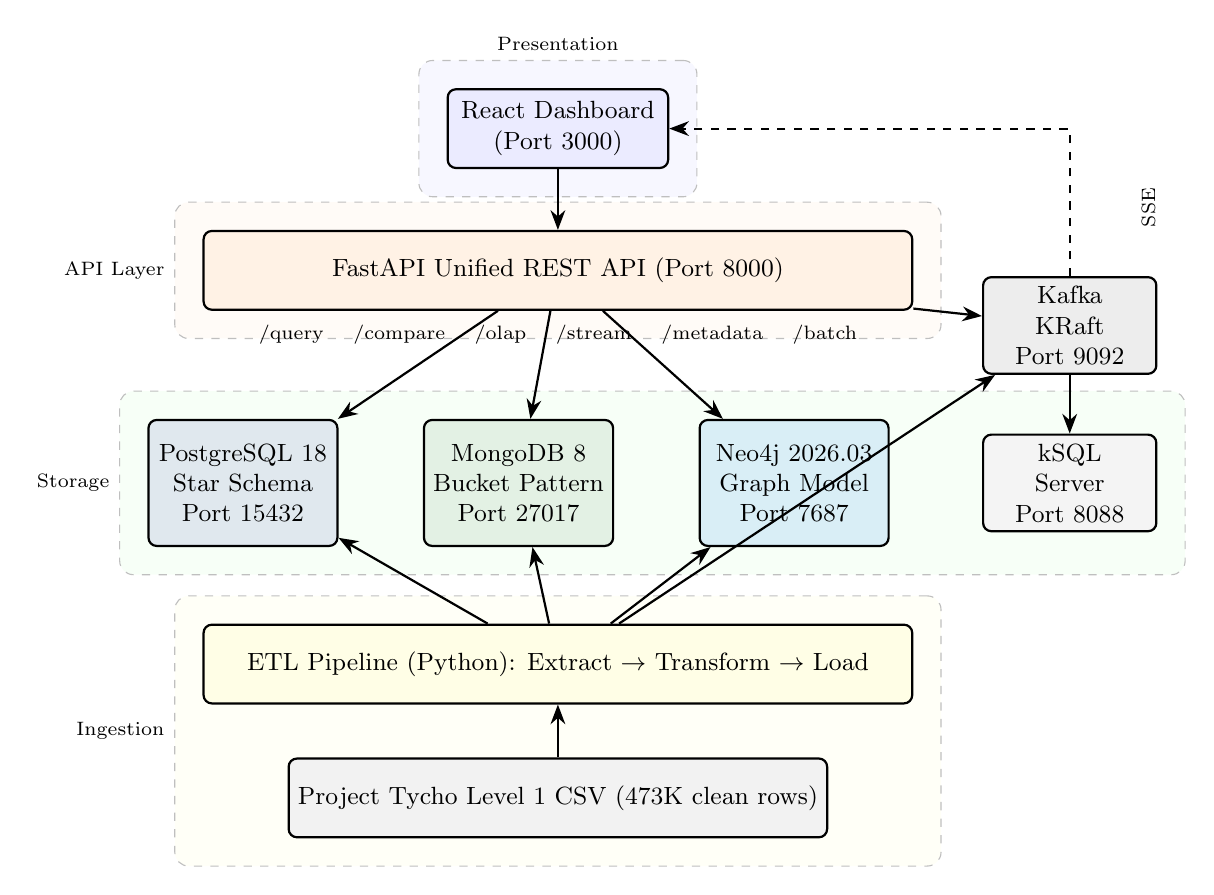
\begin{tikzpicture}[
  every node/.style={font=\small},
  box/.style={rectangle, draw, rounded corners=3pt, minimum width=2.8cm, minimum height=1cm, align=center, thick},
  dbbox/.style={box, minimum width=2.4cm, minimum height=1.6cm},
  layer/.style={rectangle, draw=gray!50, dashed, rounded corners=5pt, inner sep=10pt},
  arr/.style={-{Stealth[length=2.5mm]}, thick},
  >=Stealth
]

% Presentation layer
\node[box, fill=blue!8] (frontend) at (0, 8) {React Dashboard\\(Port 3000)};

% API layer
\node[box, fill=orange!10, minimum width=9cm] (api) at (0, 6.2) {FastAPI Unified REST API (Port 8000)};
\node[font=\scriptsize, below=0.05cm of api] {/query \quad /compare \quad /olap \quad /stream \quad /metadata \quad /batch};

% Storage layer
\node[dbbox, fill=pgblue!15] (pg) at (-4, 3.5) {PostgreSQL 18\\Star Schema\\Port 15432};
\node[dbbox, fill=mongogreen!15] (mongo) at (-0.5, 3.5) {MongoDB 8\\Bucket Pattern\\Port 27017};
\node[dbbox, fill=neoblue!15] (neo) at (3, 3.5) {Neo4j 2026.03\\Graph Model\\Port 7687};

% Streaming layer
\node[box, fill=kafkablack!8, minimum width=2.2cm] (kafka) at (6.5, 5.5) {Kafka\\KRaft\\Port 9092};
\node[box, fill=kafkablack!5, minimum width=2.2cm] (ksql) at (6.5, 3.5) {kSQL\\Server\\Port 8088};

% ETL layer
\node[box, fill=yellow!10, minimum width=9cm] (etl) at (0, 1.2) {ETL Pipeline (Python): Extract $\rightarrow$ Transform $\rightarrow$ Load};

% Data source
\node[box, fill=gray!10] (data) at (0, -0.5) {Project Tycho Level 1 CSV (473K clean rows)};

% Arrows
\draw[arr] (frontend) -- (api);
\draw[arr] (api) -- (pg);
\draw[arr] (api) -- (mongo);
\draw[arr] (api) -- (neo);
\draw[arr] (api) -- (kafka);
\draw[arr] (kafka) -- (ksql);
\draw[arr] (etl) -- (pg);
\draw[arr] (etl) -- (mongo);
\draw[arr] (etl) -- (neo);
\draw[arr] (etl) -- (kafka);
\draw[arr] (data) -- (etl);

% SSE arrow
\draw[arr, dashed] (kafka) |- (frontend);
\node[font=\scriptsize, rotate=90] at (7.5, 7) {SSE};

% Layer labels
\begin{scope}[on background layer]
  \node[layer, fill=blue!3, fit=(frontend), label={[font=\scriptsize]above:Presentation}] {};
  \node[layer, fill=orange!3, fit=(api), label={[font=\scriptsize]left:API Layer}] {};
  \node[layer, fill=green!3, fit=(pg)(mongo)(neo)(ksql), label={[font=\scriptsize]left:Storage}] {};
  \node[layer, fill=yellow!3, fit=(etl)(data), label={[font=\scriptsize]left:Ingestion}] {};
\end{scope}

\end{tikzpicture}
\caption{System architecture showing the four layers for data ingestion, storage backends, unified API, and React presentation. Kafka provides both batch ingestion and Server-Sent Events streaming to the frontend.}
\label{fig:architecture}
\end{figure}

\subsection{Service Topology}

Table~\ref{tab:services} lists all eight Docker containers and their roles. The entire system starts with a single \texttt{docker compose up} command. Health checks ensure that the backend API waits for all three databases and Kafka to become available before accepting requests.

\begin{table}[H]
\centering
\caption{Docker service topology with container names and port mappings.}
\label{tab:services}
\begin{tabular}{llrl}
\toprule
\textbf{Service} & \textbf{Container} & \textbf{Port} & \textbf{Purpose} \\
\midrule
PostgreSQL 18 & epid-postgres & 15432 & Relational star schema DW \\
MongoDB 8 & epid-mongodb & 27017 & Document-based DW (Bucket Pattern) \\
Neo4j 2026.03 & epid-neo4j & 7474/7687 & Graph-based DW with APOC \\
Kafka (KRaft) & epid-kafka & 9092 & Event streaming broker \\
ksqlDB Server & epid-ksqldb-server & 8088 & Stream processing engine \\
ksqlDB CLI & epid-ksqldb-cli & (none) & Interactive ksqlDB client \\
FastAPI & epid-backend & 8000 & Unified REST API \\
React & epid-frontend & 3000 & Analytics dashboard \\
\bottomrule
\end{tabular}
\end{table}

Kafka runs in KRaft mode, which removes the need for a separate ZooKeeper container. This reduces the total container count from nine to eight and simplifies the cluster configuration to a single environment variable block specifying the node ID, process roles, and controller quorum voters. All Kafka and ksqlDB images are pinned to Confluent Platform 8.2.0, which packages Apache Kafka 4.2.


% ================================================================
% 4. IMPLEMENTATION
% ================================================================
\section{Implementation}
\label{sec:implementation}

\subsection{PostgreSQL Star Schema}

The relational backend implements a classic Kimball star schema with three dimension tables and one fact table.

\begin{figure}[H]
\centering
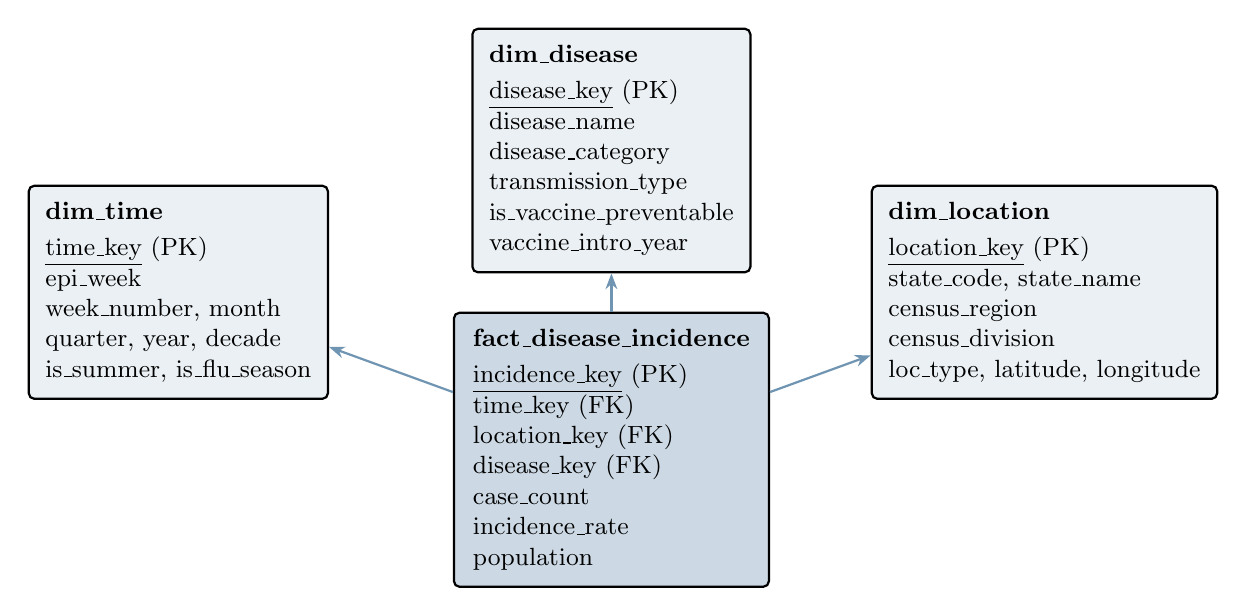
\begin{tikzpicture}[
  every node/.style={font=\small},
  dimtable/.style={rectangle, draw, thick, fill=pgblue!10, minimum width=3.5cm, align=left, inner sep=6pt, rounded corners=2pt},
  facttable/.style={rectangle, draw, thick, fill=pgblue!25, minimum width=4cm, align=left, inner sep=6pt, rounded corners=2pt},
  arr/.style={-{Stealth[length=2mm]}, thick, pgblue!70}
]

% Fact table (center)
\node[facttable] (fact) at (0, 0) {
  \textbf{fact\_disease\_incidence}\\[2pt]
  \underline{incidence\_key} (PK)\\
  time\_key (FK)\\
  location\_key (FK)\\
  disease\_key (FK)\\
  case\_count\\
  incidence\_rate\\
  population
};

% dim_time (left)
\node[dimtable] (time) at (-5.5, 2) {
  \textbf{dim\_time}\\[2pt]
  \underline{time\_key} (PK)\\
  epi\_week\\
  week\_number, month\\
  quarter, year, decade\\
  is\_summer, is\_flu\_season
};

% dim_disease (top)
\node[dimtable] (disease) at (0, 3.8) {
  \textbf{dim\_disease}\\[2pt]
  \underline{disease\_key} (PK)\\
  disease\_name\\
  disease\_category\\
  transmission\_type\\
  is\_vaccine\_preventable\\
  vaccine\_intro\_year
};

% dim_location (right)
\node[dimtable] (loc) at (5.5, 2) {
  \textbf{dim\_location}\\[2pt]
  \underline{location\_key} (PK)\\
  state\_code, state\_name\\
  census\_region\\
  census\_division\\
  loc\_type, latitude, longitude
};

% Arrows
\draw[arr] (fact) -- (time);
\draw[arr] (fact) -- (disease);
\draw[arr] (fact) -- (loc);

\end{tikzpicture}
\caption{PostgreSQL star schema with three dimension tables (time, disease, location) and one fact table containing 473{,}189 incidence records loaded from Project Tycho Level 1.}
\label{fig:starschema}
\end{figure}

The \texttt{dim\_time} table contains 4{,}947 rows, one per unique epidemiological week across the 1916--2011 time span. Derived fields support hierarchical drill-down through \texttt{week\_number}, \texttt{month}, \texttt{quarter}, \texttt{year}, \texttt{decade}, and \texttt{century}. Boolean flags for \texttt{is\_summer} and \texttt{is\_flu\_season} support seasonal filtering without date arithmetic in the queries themselves. The \texttt{dim\_location} table contains 171 rows (51 state-level entries plus 120 distinct city-level entries) and the \texttt{dim\_disease} table contains 8 rows.

A composite index on \texttt{(disease\_key, time\_key, location\_key)} covers the most common star-join access pattern. Individual foreign key indexes provide flexibility for single-dimension filtering. The schema, query planner behaviour, and materialised view refresh semantics follow the specifications documented in the PostgreSQL 18 reference manual \cite{pgdocs}. The Cypher semantics used by the Neo4j implementation in Section~\ref{sec:implementation} follow the Neo4j 2026.03 operations manual \cite{neo4jdocs}.

Four materialised views pre-aggregate the fact data at progressively coarser granularity.

\begin{enumerate}[leftmargin=2cm]
\item \texttt{mv\_monthly\_disease\_state} stores monthly case totals by disease and state. It contains 126{,}113 rows and is the finest pre-aggregation level for state-grain queries.
\item \texttt{mv\_yearly\_disease\_region} stores yearly totals by disease and census region with peak weekly case tracking, totalling 1{,}253 rows.
\item \texttt{mv\_decade\_disease\_national} stores decade-level national totals (46 rows), the coarsest roll-up.
\item \texttt{mv\_yearly\_disease\_city} stores yearly city-level totals (3{,}301 rows). It exists specifically to serve city-grain queries against the diphtheria portion of the dataset.
\end{enumerate}

These views are created \texttt{WITH NO DATA} in the initialisation script and populated with \texttt{REFRESH MATERIALIZED VIEW} after the fact table is loaded. The total PostgreSQL database size after loading the cleaned Project Tycho Level 1 dataset is 92~MB, of which \texttt{fact\_disease\_incidence} accounts for 66~MB and the four materialised views together account for roughly 17.4~MB.

\subsection{MongoDB Document Model}

The MongoDB implementation uses the Bucket Pattern to store the same data as embedded documents. Each document represents one month of observations for a specific disease and reporting location. The document structure is shown below.

\begin{lstlisting}[language={}, caption={MongoDB bucket document structure (simplified).}, label={lst:mongodoc}]
{
  "disease": { "name": "MEASLES", "category": "Viral",
               "vaccine_year": 1963 },
  "location": { "state_code": "CA", "state_name": "CALIFORNIA",
                 "loc": "CALIFORNIA", "loc_type": "STATE",
                 "region": "West" },
  "time_bucket": { "year": 1960, "month": 3, "decade": 1960 },
  "weekly_observations": [
    { "epi_week": 196009, "cases": 1247, "incidence_rate": 7.93 },
    { "epi_week": 196010, "cases": 1389, "incidence_rate": 8.83 }
  ],
  "monthly_summary": {
    "total_cases": 5604, "avg_incidence_rate": 8.91,
    "peak_weekly_cases": 1512, "observation_count": 4
  }
}
\end{lstlisting}

This design embeds dimension attributes directly into each document, removing the need for joins. The \texttt{monthly\_summary} sub-document provides pre-computed aggregates at the document level, so queries that operate at monthly granularity or coarser do not need to unwind the weekly observations array.

The primary collection contains 155{,}063 bucket documents, with an average of 3.05 weekly observations per bucket. Two pre-aggregated collections are populated through aggregation pipelines that use the \texttt{\$merge} stage. The first, \texttt{summary\_monthly\_by\_region}, contains 14{,}158 documents and aggregates state-grain observations at monthly granularity by census region. The second, \texttt{summary\_decade\_national}, contains 46 documents and provides decade-level national totals.

Compound indexes on \texttt{(disease.name, time\_bucket.year, location.state\_code)} and \texttt{(location.region, time\_bucket.decade)} match the primary query access patterns. A separate index on \texttt{(location.loc\_type, location.loc)} accelerates the city-grain queries used for diphtheria.

\subsection{Neo4j Graph Model}

The graph implementation models dimension hierarchies as chains of nodes connected by typed relationships, with observation data stored as intermediate nodes linking dimension endpoints.

\begin{figure}[H]
\centering
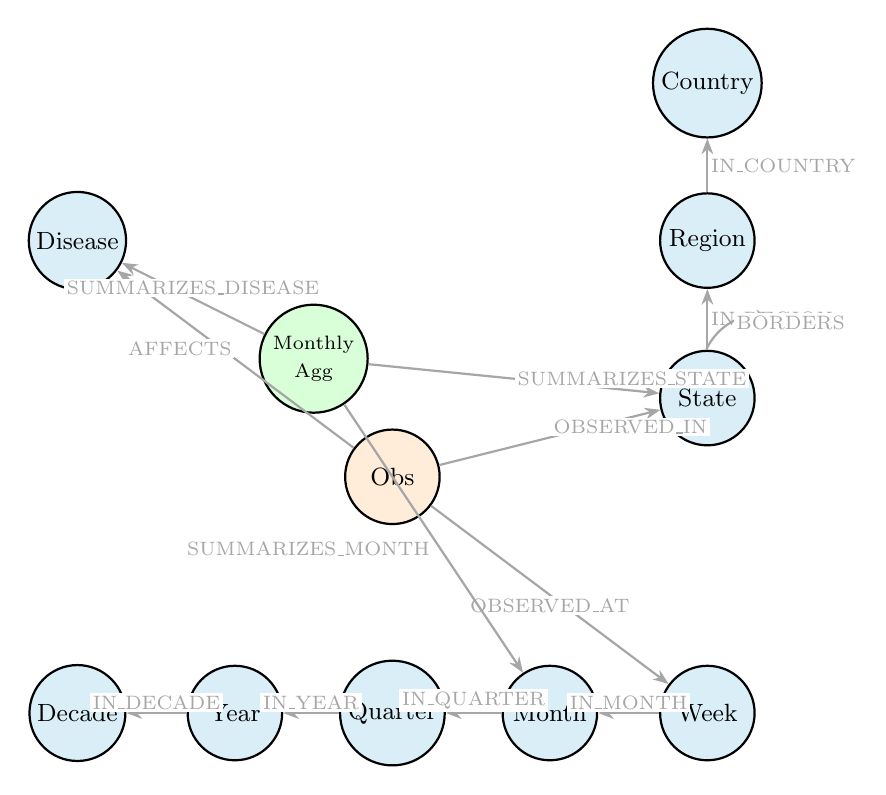
\begin{tikzpicture}[
  every node/.style={font=\small},
  node/.style={circle, draw, thick, minimum size=1.2cm, align=center, inner sep=2pt},
  gnode/.style={node, fill=neoblue!15},
  onode/.style={node, fill=orange!15},
  anode/.style={node, fill=green!15},
  rel/.style={-{Stealth[length=2mm]}, thick, gray!70},
  rlabel/.style={font=\scriptsize, midway, fill=white, inner sep=1pt}
]

% Disease
\node[gnode] (disease) at (-4, 3) {Disease};
% Location hierarchy
\node[gnode] (country) at (4, 5) {Country};
\node[gnode] (region) at (4, 3) {Region};
\node[gnode] (state) at (4, 1) {State};
% Time hierarchy
\node[gnode] (decade) at (-4, -3) {Decade};
\node[gnode] (year) at (-2, -3) {Year};
\node[gnode] (quarter) at (0, -3) {Quarter};
\node[gnode] (month) at (2, -3) {Month};
\node[gnode] (week) at (4, -3) {Week};

% Central nodes
\node[onode] (obs) at (0, 0) {Obs};
\node[anode] (agg) at (-1, 1.5) {\scriptsize Monthly\\[-1pt]\scriptsize Agg};

% Relationships
\draw[rel] (obs) -- node[rlabel, above left] {AFFECTS} (disease);
\draw[rel] (obs) -- node[rlabel, above right] {OBSERVED\_IN} (state);
\draw[rel] (obs) -- node[rlabel, below] {OBSERVED\_AT} (week);

\draw[rel] (agg) -- node[rlabel, above] {\scriptsize SUMMARIZES\_DISEASE} (disease);
\draw[rel] (agg) -- node[rlabel, right] {\scriptsize SUMMARIZES\_STATE} (state);
\draw[rel] (agg) -- node[rlabel, below left] {\scriptsize SUMMARIZES\_MONTH} (month);

\draw[rel] (state) -- node[rlabel, right] {IN\_REGION} (region);
\draw[rel] (region) -- node[rlabel, right] {IN\_COUNTRY} (country);
\draw[rel] (week) -- node[rlabel, above] {IN\_MONTH} (month);
\draw[rel] (month) -- node[rlabel, above] {IN\_QUARTER} (quarter);
\draw[rel] (quarter) -- node[rlabel, above] {IN\_YEAR} (year);
\draw[rel] (year) -- node[rlabel, above] {IN\_DECADE} (decade);

% Border self-relationship
\draw[rel, bend left=40] (state) to node[rlabel, right] {BORDERS} ++(0.8, 1);

\end{tikzpicture}
\caption{Neo4j graph model showing node types (circles) and relationship types (arrows). Observation nodes link to Disease, State, and Week nodes. MonthlyAggregate nodes provide pre-computed summaries linked to Disease, State, and Month.}
\label{fig:graphmodel}
\end{figure}

The graph contains 473{,}189 Observation nodes and 139{,}683 MonthlyAggregate nodes. The aggregate count is lower than the MongoDB bucket count (155{,}063) because the Neo4j loader attaches the MonthlyAggregate nodes only to state-grain observations and the city-grain diphtheria series is summarised separately through the \texttt{LOCATED\_IN\_STATE} relationship. The time hierarchy chain (Week $\rightarrow$ Month $\rightarrow$ Quarter $\rightarrow$ Year $\rightarrow$ Decade) contains 6{,}590 nodes and, together with the geographic hierarchy and Disease nodes, the total dimension and hierarchy node count is 6{,}774. The spatial \texttt{BORDERS} relationship between State nodes comprises 214 directed edges across the 48 contiguous states and is unique to the graph model. It enables three graph-exclusive queries (Q11, Q12, Q13) that cannot be expressed naturally in SQL or in MongoDB aggregation pipelines.

City-level diphtheria observations are represented as an additional set of 120 City nodes, each connected to its parent State through a typed \texttt{LOCATED\_IN\_STATE} relationship. The ETL distinguishes the two grains by attaching state-grain observations with \texttt{OBSERVED\_IN} and city-grain observations with \texttt{OBSERVED\_IN\_CITY}. The MonthlyAggregate layer rolls both grains into the same per-disease, per-state, per-month summary by using an \texttt{OPTIONAL MATCH} coalesce pattern.

The MonthlyAggregate nodes carry \texttt{total\_cases}, \texttt{avg\_incidence}, and \texttt{observation\_count} properties. Most analytical queries (Q1 through Q10) are routed through these aggregate nodes rather than the raw Observation nodes, which reduces the traversal scope by roughly a factor of 3.05.

\subsection{Kafka Streaming Pipeline}

The streaming subsystem consists of a Kafka producer, four kSQL stream and table definitions, and a Server-Sent Events (SSE) consumer.

\begin{figure}[H]
\centering
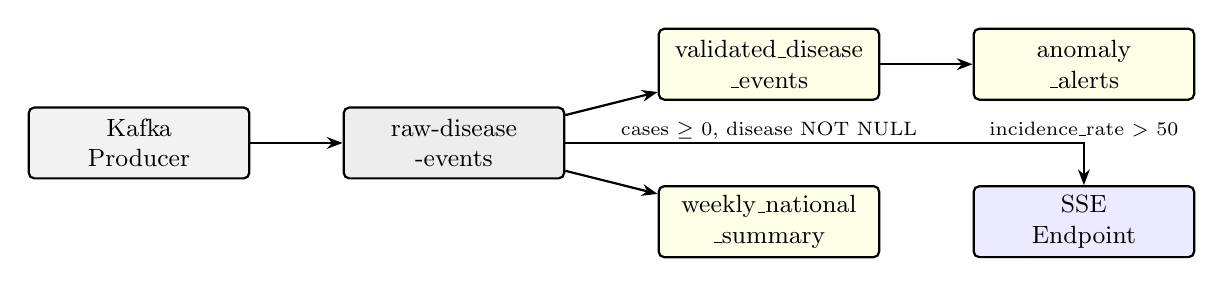
\begin{tikzpicture}[
  every node/.style={font=\small},
  box/.style={rectangle, draw, thick, rounded corners=2pt, minimum width=2.8cm, minimum height=0.9cm, align=center},
  topic/.style={box, fill=kafkablack!8},
  stream/.style={box, fill=yellow!10},
  arr/.style={-{Stealth[length=2mm]}, thick},
]

\node[box, fill=gray!10] (producer) at (-4, 0) {Kafka\\Producer};
\node[topic] (raw) at (0, 0) {raw-disease\\-events};
\node[stream] (validated) at (4, 1) {validated\_disease\\\_events};
\node[stream] (summary) at (4, -1) {weekly\_national\\\_summary};
\node[stream] (anomaly) at (8, 1) {anomaly\\\_alerts};
\node[box, fill=blue!8] (sse) at (8, -1) {SSE\\Endpoint};

\draw[arr] (producer) -- (raw);
\draw[arr] (raw) -- (validated);
\draw[arr] (raw) -- (summary);
\draw[arr] (validated) -- (anomaly);
\draw[arr] (raw) -| (sse);

\node[font=\scriptsize, below=0.15cm of validated] {cases $\geq$ 0, disease NOT NULL};
\node[font=\scriptsize, below=0.15cm of anomaly] {incidence\_rate $>$ 50};

\end{tikzpicture}
\caption{Kafka streaming pipeline. Raw events are validated by kSQL, aggregated into a windowed table, and filtered for anomaly detection. The SSE endpoint streams events to the React frontend.}
\label{fig:kafka_pipeline}
\end{figure}

The producer reads the CSV file and publishes each row as a JSON message with configurable throughput delay. Messages are keyed by \texttt{state\_epi\_week} to ensure per-state ordering within partitions.

kSQL defines four processing stages: (1) \texttt{disease\_events\_stream} reads from the raw topic with a JSON schema declaration, (2) \texttt{validated\_disease\_events} filters out null diseases and negative case counts, (3) \texttt{weekly\_national\_summary} computes a grouped aggregation of national cases by disease and epidemiological week, and (4) \texttt{anomaly\_alerts} flags any validated event with an incidence rate exceeding 50 per 100,000.

\subsection{Unified API Layer}

The FastAPI backend exposes endpoints organized into six router modules. Table~\ref{tab:endpoints} summarizes the API surface.

\begin{table}[H]
\centering
\caption{REST API endpoint summary.}
\label{tab:endpoints}
\begin{tabular}{lll}
\toprule
\textbf{Method} & \textbf{Endpoint} & \textbf{Description} \\
\midrule
GET & /api/v1/health & Backend connectivity status \\
GET & /api/v1/queries & List all 13 queries with metadata \\
POST & /api/v1/query & Execute query on one backend \\
POST & /api/v1/compare & Run query on all backends concurrently \\
POST & /api/v1/olap/\{op\} & OLAP operations (slice, dice, etc.) \\
GET & /api/v1/metadata/\{backend\} & Schema introspection \\
POST & /api/v1/batch/refresh-summaries & Refresh materialized views \\
GET & /api/v1/stream/events & SSE real-time Kafka events \\
\bottomrule
\end{tabular}
\end{table}

The comparison endpoint is the most architecturally significant. When a client sends a query ID and optional parameters, the handler dispatches the same logical query to all three backends concurrently using a \texttt{ThreadPoolExecutor} with three workers. Each worker calls the corresponding service method, measures execution time, captures the native query text (SQL, aggregation pipeline JSON, or Cypher), and returns the results. The client receives a single response containing three sub-objects:

\begin{lstlisting}[language={}, caption={Comparison endpoint response structure.}]
{
  "query_id": "Q1",
  "backends": {
    "postgres": { "results": [...], "execution_time_ms": 799,
                  "query_text": "SELECT d.disease_name..." },
    "mongodb":  { "results": [...], "execution_time_ms": 1853,
                  "query_text": "[{\"$group\": ...}]" },
    "neo4j":    { "results": [...], "execution_time_ms": 1624,
                  "query_text": "MATCH (a:Monthly..." }
  }
}
\end{lstlisting}

\subsection{Query Implementation Strategy}

Each of the 10 cross-backend queries is implemented natively in the query language of each database. The implementations are not transliterations; they exploit each backend's strengths.

PostgreSQL queries use CTEs, window functions (\texttt{LAG}, \texttt{RANK}, \texttt{STDDEV}), \texttt{LATERAL} joins (for Q8's vaccination impact comparison), and \texttt{CORR} aggregate (for Q6's co-occurrence correlation).

MongoDB queries use aggregation pipelines with stages including \texttt{\$group}, \texttt{\$unwind}, \texttt{\$match}, \texttt{\$setWindowFields} (for Q5's year-over-year shift), and \texttt{\$stdDevPop} (for Q9's z-score calculation). The Q6 co-occurrence query uses a simplified approach that counts per-disease frequency in state-years with multiple active diseases, rather than computing pairwise correlations as PostgreSQL does. This represents a conscious trade-off, because the aggregation pipeline does not have a native correlation function, so the implementation prioritizes what the framework does well rather than forcing an awkward emulation.

Neo4j queries use \texttt{MATCH} patterns with multi-hop traversal through the time hierarchy, \texttt{CALL} subqueries (for Q8's pre/post vaccine comparison), \texttt{COLLECT} with \texttt{UNWIND} and \texttt{RANGE} (for Q5's year-over-year calculation), and \texttt{stDev} aggregation (for Q9's anomaly detection).

Three graph-exclusive queries (Q11, Q12, Q13) run only on Neo4j. Q11 traverses \texttt{BORDERS} relationships between states to detect temporal lags in disease spread between neighbors. Q12 computes a disease composition profile for each state as a percentage breakdown. Q13 measures each disease's geographic coverage as a fraction of total state-year combinations with significant case counts.


% ================================================================
% 5. DATA AND PREPROCESSING
% ================================================================
\section{Data and Preprocessing}
\label{sec:data}

\subsection{Source Data}

The primary data source is the Project Tycho Level 1 release from the University of Pittsburgh \cite{vanpanhuis2013, vanpanhuis2018}, available through the Project Tycho data portal \cite{tychoportal}. The CSV file (\texttt{data/raw/tycho\_level1\_real.csv}) contains 759{,}467 raw rows, of which 473{,}189 carry positive case counts after cleaning. Cleaning drops rows with non-numeric or zero case counts, normalises disease names to uppercase, and rejects rows missing a state or disease label.

Each row carries seven columns: \texttt{epi\_week} (YYYYWW format), \texttt{state} (two-letter code), \texttt{loc} (location name), \texttt{loc\_type} (STATE or CITY), \texttt{disease} (uppercase name), \texttt{cases} (integer), and \texttt{incidence\_per\_100000} (float). Seven of the eight diseases (measles, pertussis, polio, hepatitis A, mumps, rubella, smallpox) are reported at state granularity. Diphtheria is reported only at city granularity over the years 1916--1947, covering 120 distinct (state, city) pairs across 116 unique city names. The full cleaned dataset spans 1916--2011, contains 4{,}947 distinct epidemiological weeks, covers 51 state-level jurisdictions (the 50 states plus the District of Columbia), and totals 24{,}878{,}333 reported cases. The Tycho Level 1 dataset card on the Project Tycho portal states the canonical range as 1916--2009 across 50 states and 122 cities. The downloaded flat file used in this project carries a 6{,}566-row residual tail of pertussis and hepatitis A rows from calendar years 2010 and 2011 and, after cleaning, resolves to 120 distinct (state, city) pairs across 116 unique city names and to the 51 state-level jurisdictions listed above (the 50 states plus the District of Columbia, which the portal groups under its 50-state count). All figures, tables and benchmark timings in this report are computed on the full cleaned file as loaded, so the 2010--2011 tail is included wherever it contributes (notably the pivot table 2010s row and the 4{,}947 distinct epidemiological weeks count).

In parallel with the real dataset, this project ships a synthetic generator (\texttt{etl/generate\_synthetic\_data.py}) that produces records matching the same schema and statistical characteristics. The synthetic data is retained as a reproducible benchmark to compare load and query performance against a controllable distribution. All section~\ref{sec:results} measurements are taken on the real Project Tycho Level 1 data unless explicitly labelled as synthetic.

\subsection{Synthetic Benchmark Generation Model}

The synthetic generator is used only for controlled benchmarking and is not the source of any numeric result in Section~\ref{sec:results}. Its expected weekly case count for disease $d$, state $s$, year $y$, and week $w$ is computed as:

\begin{equation}
\label{eq:expected}
E(d, s, y, w) = B_d \cdot \frac{P(s, y)}{100{,}000} \cdot S(d, w) \cdot V(d, y) \cdot D(d, y)
\end{equation}

where $B_d$ is the base weekly rate per 100,000 for disease $d$, $P(s, y)$ is the interpolated population of state $s$ in year $y$, $S(d, w)$ is the seasonal modulation factor, $V(d, y)$ is the vaccine effect, and $D(d, y)$ is a post-vaccine decade-based scaling factor (equal to 1 before the vaccine introduction year).

The seasonal modulation follows a cosine function centered on the disease-specific peak week $w_p$:

\begin{equation}
S(d, w) = 1 + A_d \cdot \cos\!\left(\frac{2\pi(w - w_p)}{52}\right)
\end{equation}

where $A_d$ is the seasonal amplitude. Respiratory diseases like measles peak in late winter ($w_p = 12$), while polio peaks in summer ($w_p = 32$).

For most diseases, the vaccine effect applies an exponential decay after the vaccine introduction year $y_v$:

\begin{equation}
V(d, y) = \begin{cases} 1 & \text{if } y \leq y_v \\ e^{-\lambda_d (y - y_v)} & \text{if } y > y_v \end{cases}
\end{equation}

where $\lambda_d$ is a disease-specific decay constant. Smallpox is treated as a special case in the generator. Because its vaccine was introduced in 1796, well before the modern reporting era, the code applies a linear decline toward zero over the first half of the twentieth century, reflecting the historical eradication trajectory rather than the exponential decay model.

Actual case counts are drawn from a Poisson distribution with parameter $E(d, s, y, w)$, giving each observation realistic integer-valued noise. Rows with zero cases are excluded from the output.

\begin{table}[H]
\centering
\caption{Disease generation parameters. Base rate is per 100,000 per week.}
\label{tab:disease_params}
\begin{tabular}{lrrrcr}
\toprule
\textbf{Disease} & \textbf{Base Rate} & \textbf{Seasonal Amp.} & \textbf{Peak Week} & \textbf{Vaccine Year} & $\boldsymbol{\lambda}$ \\
\midrule
Measles & 4.0 & 0.6 & 12 & 1963 & 0.15 \\
Pertussis & 1.5 & 0.3 & 28 & 1948 & 0.10 \\
Polio & 0.8 & 0.7 & 32 & 1955 & 0.25 \\
Diphtheria & 1.2 & 0.4 & 8 & 1923 & 0.08 \\
Smallpox & 0.5 & 0.3 & 10 & 1796 & * \\
Hepatitis A & 0.6 & 0.2 & 42 & 1995 & 0.12 \\
Mumps & 1.0 & 0.5 & 14 & 1967 & 0.13 \\
Rubella & 0.9 & 0.5 & 16 & 1969 & 0.18 \\
\bottomrule
\end{tabular}
\vspace{0.3em}
\raggedright\small *Smallpox uses a linear decline model rather than the exponential decay applied to other diseases.
\end{table}

\subsection{Reference Data}

Four reference CSV files supplement both the real and the synthetic data.

\textbf{us\_regions.csv} maps 51 state codes (the 50 states plus the District of Columbia) to full state names, Census regions (Northeast, Midwest, South, West), Census divisions (for example Middle Atlantic, Pacific), and geographic coordinates. The District of Columbia is included because Project Tycho Level 1 reports DC separately for hepatitis A, mumps, and rubella.

\textbf{disease\_metadata.csv} defines the eight diseases with their epidemiological category (Viral or Bacterial), transmission mode (Airborne, Fecal-oral, Contact), vaccine preventability, and the year the US vaccine was introduced.

\textbf{state\_populations.csv} provides 561 population estimates, one per (state, decade) combination, for all 51 jurisdictions at each decadal Census from 1910 through 2010. The decade grid encloses the 1916--2011 dataset range on both ends (the 2011 year is extrapolated from the 2010 Census anchor). Of the 561 rows, 461 carry \texttt{source=census} and 100 carry \texttt{source=extrapolated\_from\_1930\_1940}; the extrapolated rows cover the 1910 and 1920 decades for the 50 jurisdictions whose first Census-published figure in this file is 1930. The remaining jurisdiction is Census-sourced across all 11 decade anchors. Between Census anchor points the loader interpolates linearly to estimate per-year population.

\textbf{state\_borders.csv} lists the border adjacency for each of the 48 contiguous states (Alaska and Hawaii are excluded because they share no land borders). The file is used to create the 214 \texttt{BORDERS} relationships in Neo4j.

\subsection{ETL Pipeline}

The ETL pipeline proceeds through four stages. The \texttt{extract.py} module reads all CSV files into pandas DataFrames. The \texttt{transform.py} module performs cleaning (dropping rows with null or non-positive cases, normalising disease names to uppercase), derives time dimension fields from epidemiological week numbers, builds the three target structures (star schema DataFrames, MongoDB bucket documents, Neo4j node and relationship lists) and assigns surrogate keys. The three loader scripts (\texttt{load\_postgres.py}, \texttt{load\_mongo.py}, \texttt{load\_neo4j.py}) write the transformed data into their respective backends. A single environment variable, \texttt{TYCHO\_DATA\_FILE}, switches the pipeline between the real Project Tycho Level 1 file and the synthetic benchmark file, with no other code changes required.

The PostgreSQL loader uses the \texttt{COPY} protocol through \texttt{psycopg2} for maximum insert throughput. The MongoDB loader uses \texttt{insert\_many} with batches of 10{,}000 documents. The Neo4j loader uses \texttt{UNWIND} batch queries with batches of 5{,}000 observation records and branches on \texttt{loc\_type} so that state-grain rows attach with \texttt{OBSERVED\_IN} while city-grain rows attach with \texttt{OBSERVED\_IN\_CITY}.

\begin{figure}[H]
\centering
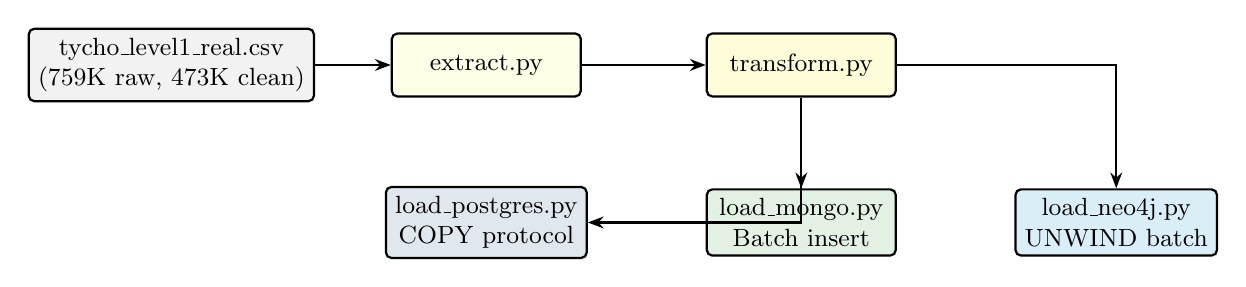
\begin{tikzpicture}[
  every node/.style={font=\small},
  box/.style={rectangle, draw, thick, rounded corners=2pt, minimum width=2.4cm, minimum height=0.8cm, align=center},
  arr/.style={-{Stealth[length=2mm]}, thick},
]

\node[box, fill=gray!10] (csv) at (0, 0) {tycho\_level1\_real.csv\\(759K raw, 473K clean)};
\node[box, fill=yellow!10] (extract) at (4, 0) {extract.py};
\node[box, fill=yellow!15] (transform) at (8, 0) {transform.py};

\node[box, fill=pgblue!15] (pg) at (4, -2) {load\_postgres.py\\COPY protocol};
\node[box, fill=mongogreen!15] (mongo) at (8, -2) {load\_mongo.py\\Batch insert};
\node[box, fill=neoblue!15] (neo) at (12, -2) {load\_neo4j.py\\UNWIND batch};

\draw[arr] (csv) -- (extract);
\draw[arr] (extract) -- (transform);
\draw[arr] (transform) |- (pg);
\draw[arr] (transform) -- (mongo);
\draw[arr] (transform) -| (neo);

\end{tikzpicture}
\caption{ETL pipeline from raw CSV through extraction, transformation, and backend-specific loading.}
\label{fig:etl_pipeline}
\end{figure}


% ================================================================
% 6. RESULTS / EVALUATION
% ================================================================
\section{Results and Evaluation}
\label{sec:results}

\subsection{Data Volume Verification}

After loading the real Project Tycho Level 1 dataset, the three backends contain the data volumes shown in Table~\ref{tab:data_volumes}. The fact count is consistent across all backends at 473{,}189 observations. MongoDB's primary collection holds 155{,}063 bucket documents at an average of 3.05 weekly observations per bucket. Neo4j's Observation node count matches the PostgreSQL fact count because each observation is stored as an individual node.

\begin{table}[H]
\centering
\caption{Data volumes across the three backends after loading Project Tycho Level 1 (473{,}189 clean fact rows, 1916--2011). All three sizes are measured on the live Docker deployment: PostgreSQL via \texttt{pg\_database\_size}, MongoDB via \texttt{dbStats.dataSize}, Neo4j via the store file size in \texttt{/data/databases/neo4j}.}
\label{tab:data_volumes}
\begin{tabular}{lrrr}
\toprule
\textbf{Metric} & \textbf{PostgreSQL} & \textbf{MongoDB} & \textbf{Neo4j} \\
\midrule
Primary fact / document / node count & 473{,}189 & 155{,}063 & 473{,}189 \\
Dimension or hierarchy entities & 4{,}947 + 171 + 8 & (embedded) & 6{,}774 nodes \\
Pre-aggregated summaries & 4 mat. views & 2 collections & 139{,}683 agg. nodes \\
Diseases & 8 & 8 & 8 \\
State-level jurisdictions & 51 & 51 & 51 \\
City-level jurisdictions & 120 & 120 & 120 \\
Time span (years) & 1916--2011 & 1916--2011 & 1916--2011 \\
Database size & 92 MB & 114 MB & 103 MB \\
\bottomrule
\end{tabular}
\end{table}

The PostgreSQL footprint breaks down as 66~MB for \texttt{fact\_disease\_incidence} (31~MB heap plus 35~MB in the composite and per-dimension indexes), 17~MB for \texttt{mv\_monthly\_disease\_state}, 296~KB for \texttt{mv\_yearly\_disease\_city}, 160~KB for \texttt{mv\_yearly\_disease\_region} and 24~KB for \texttt{mv\_decade\_disease\_national}. The three dimension tables occupy 584~KB, 80~KB and 40~KB for \texttt{dim\_time}, \texttt{dim\_location} and \texttt{dim\_disease} respectively. A full end-to-end load from the cleaned CSV into PostgreSQL, including all index builds and the refresh of the four materialised views, completes in approximately 163 seconds on a modest laptop-class environment.

The MongoDB footprint is dominated by the primary \texttt{disease\_observations} collection at 112~MB across 155{,}063 bucket documents with an average document size of 754~bytes, reflecting the embedded dimension attributes and the weekly observation array. The pre-aggregated \texttt{summary\_monthly\_by\_region} collection adds 2~MB across 14{,}158 documents with an average document size of 143~bytes, and \texttt{summary\_decade\_national} holds 46 documents in under 10~KB. The remainder of the 114~MB total is absorbed by the compound indexes on \texttt{(disease.name, time\_bucket.year, location.state\_code)}, \texttt{(location.region, time\_bucket.decade)} and \texttt{(location.loc\_type, location.loc)}, plus the default \texttt{\_id} index on every collection.

The Neo4j store is dominated by the relationship store at 64~MB, followed by the property store at 24~MB and the node store at 9~MB, with the remaining 6~MB spread across schema indexes, the relationship-group store and the token stores. The relationship store is the single largest component because every \texttt{OBSERVED\_IN}, \texttt{AFFECTS}, \texttt{OBSERVED\_AT}, \texttt{OBSERVED\_IN\_CITY} and \texttt{SUMMARIZES\_*} edge is a fixed-width record and the graph contains 1{,}845{,}584 such edges across fifteen relationship types. The 619{,}646 nodes and their properties occupy the node and property stores, which together account for 33~MB.

\subsection{Query Performance Comparison}

Table~\ref{tab:query_perf} reports execution times for the ten cross-backend queries measured on the real Project Tycho Level 1 dataset in every backend. Each cell is the median of seven consecutive runs against a warm cache with the first two runs dropped as warmup. The 25th and 75th percentiles bracket the remaining five runs and quantify the measurement noise. All three backends run in Docker Desktop containers on the same host (Windows 11, 8~GB RAM allocated to Docker, SSD storage) and the client is a FastAPI worker in the backend container, so each timing covers driver round-trip plus execution but not host-to-container network overhead.

\begin{table}[H]
\centering
\caption{Query execution times on the real Project Tycho Level 1 dataset (473{,}189 rows), in milliseconds. For each query and backend the cell shows the median followed by the 25th and 75th percentile of five timed runs (seven runs, two warmup runs dropped). Lower is better in each row.}
\label{tab:query_perf}
\resizebox{\textwidth}{!}{%
\begin{tabular}{clrrr}
\toprule
\textbf{ID} & \textbf{Query (abbreviated)} & \textbf{PostgreSQL} & \textbf{MongoDB} & \textbf{Neo4j} \\
\midrule
Q1  & Cases by disease and decade        &  250.75 {\footnotesize [222.07, 267.86]} &  147.69 {\footnotesize [140.44, 160.05]} &  527.18 {\footnotesize [451.34, 568.17]} \\
Q2  & Measles by state (1960)            &   17.79 {\footnotesize [17.49,  18.01]}  &    5.63 {\footnotesize [5.36,   5.81]}   &   11.38 {\footnotesize [11.00, 13.95]}  \\
Q3  & Top 10 states (Measles, 1950--70)  &   54.61 {\footnotesize [53.64,  55.64]}  &   21.92 {\footnotesize [21.50,  23.73]}  &  117.92 {\footnotesize [90.32, 130.09]} \\
Q4  & Seasonal pattern (Measles)         &   86.16 {\footnotesize [83.64,  88.75]}  &  242.91 {\footnotesize [233.76, 243.28]} &  103.39 {\footnotesize [100.52, 104.72]} \\
Q5  & Year-over-year change              &  171.34 {\footnotesize [129.56, 172.94]} &  126.51 {\footnotesize [105.66, 144.36]} &  417.15 {\footnotesize [381.12, 459.03]} \\
Q6  & Disease co-occurrence              &  328.51 {\footnotesize [314.40, 334.33]} &  270.74 {\footnotesize [252.13, 345.88]} &  641.65 {\footnotesize [620.23, 661.78]} \\
Q7  & Geographic spread ranking          &  118.00 {\footnotesize [111.80, 120.43]} &   94.76 {\footnotesize [85.37,  99.15]}  &  206.02 {\footnotesize [172.72, 212.84]} \\
Q8  & Vaccination impact                 &  147.18 {\footnotesize [141.03, 149.70]} &  200.72 {\footnotesize [190.17, 207.98]} &  428.91 {\footnotesize [411.74, 555.26]} \\
Q9  & Anomaly detection (z-score)        &  575.59 {\footnotesize [523.86, 582.18]} &  298.41 {\footnotesize [263.33, 302.67]} & 1{,}132.68 {\footnotesize [770.93, 1{,}487.55]} \\
Q10 & Normalised trend comparison        &  266.13 {\footnotesize [215.68, 323.77]} &  178.15 {\footnotesize [174.13, 206.08]} &  385.21 {\footnotesize [343.78, 436.97]} \\
\bottomrule
\end{tabular}%
}
\vspace{0.3em}
\raggedright\small All thirty cells in the Q1--Q10 $\times$ \{PostgreSQL, MongoDB, Neo4j\} grid are measured on the same real Project Tycho Level 1 load. The three backends return matching row counts on Q1, Q2, Q3, Q4 and Q7. Four queries return non-identical row counts. Q5 returns 3{,}257 rows on PostgreSQL and MongoDB and 3{,}206 rows on Neo4j; the 51-row gap matches the 51 state-level jurisdictions whose first reported year has no prior year in the Neo4j lag-window scheme. Q6 returns 15 rows on PostgreSQL, 8 on MongoDB and 19 on Neo4j and is discussed below. Q8 returns 8 rows on PostgreSQL and 7 on MongoDB and Neo4j; PostgreSQL retains smallpox (vaccine year 1796) through its \texttt{LATERAL} join even though the pre-vaccine window falls outside the dataset, while the MongoDB and Neo4j implementations guard with \texttt{vaccine\_year $\geq$ 1900} and exclude it. Q10 returns 315 rows on PostgreSQL and 347 on MongoDB and Neo4j; the difference corresponds to city-grain diphtheria years that the PostgreSQL query filters out with \texttt{loc\_type = 'STATE'} and that the MongoDB and Neo4j implementations include.
\end{table}

The relative ordering of the three backends varies across the ten queries. MongoDB wins on Q1, Q2, Q3, Q5, Q6, Q7, Q9, and Q10, all of which benefit from the denormalised bucket documents and the compound indexes on \texttt{(disease.name, time\_bucket.year, location.state\_code)}. On Q2, the single-disease single-year slice, MongoDB completes in a median of 5.63~ms through a direct index seek, against PostgreSQL's 17.79~ms star join and Neo4j's 11.38~ms multi-hop traversal. On Q9, which computes a national standard deviation in the pre-aggregated \texttt{summary\_decade\_national} collection, MongoDB at 298~ms is almost twice as fast as PostgreSQL's 575~ms because the z-score computation fits in a single aggregation pipeline without touching the large fact collection.

PostgreSQL wins on Q4 and Q8. Q4 is the seasonal-pattern roll-up, where PostgreSQL's star join on \texttt{fact\_disease\_incidence}, \texttt{dim\_time}, and \texttt{dim\_disease} completes in 86~ms with the composite index on \texttt{(disease\_key, time\_key, location\_key)}. The MongoDB equivalent has to \texttt{\$unwind} the weekly observation array inside each bucket document to recover weekly granularity, which costs 243~ms. Q8 is the vaccination impact query; PostgreSQL executes it as a \texttt{LATERAL} join that emits one row per disease and computes both the pre-vaccine and post-vaccine average in a single scan of the fact table, finishing in 147~ms. The MongoDB implementation runs two independent aggregations per disease (eight diseases total) and pays the per-aggregation overhead on each, finishing in 201~ms.

Neo4j is the slowest backend on every query. The shortest timings (Q2 at 11.38~ms and Q1 at 527~ms) are still longer than the corresponding PostgreSQL and MongoDB timings on the same query, and the gap widens on broad aggregations (Q9 at 1{,}133~ms against MongoDB's 298~ms). The cost is inherent in the graph model for non-traversal OLAP queries: every decade-level aggregate must walk the Month $\rightarrow$ Quarter $\rightarrow$ Year $\rightarrow$ Decade chain, and every state filter must follow an \texttt{OBSERVED\_IN} edge. Neo4j's value on this dataset is not visible in Q1--Q10 but in the graph-only queries Q11--Q13 discussed in Section~\ref{sec:graphonly}.

The one query where the three backends return different row counts is Q6, which counts disease pairs that spike together in the same state-year. PostgreSQL returns 15 rows using the built-in \texttt{CORR} aggregate with a 0.5 Pearson correlation threshold. MongoDB lacks a correlation aggregator and the project's pipeline uses a simplified per-disease co-occurrence count with a distinct-state threshold, returning 8 rows. Neo4j uses a pattern match on (Observation)-[:OBSERVED\_IN]->(State)<-[:OBSERVED\_IN]-(Observation) and returns 19 rows. The three implementations answer a related but non-identical question and this is the sole case in the ten-query grid where the row counts do not match.

\subsubsection{Graph-Only Queries (Q11--Q13)}
\label{sec:graphonly}

Table~\ref{tab:query_graph_only} reports measured timings for the three Neo4j-only queries. Q11 traces disease spread between neighbouring states along the \texttt{BORDERS} edge and is by far the most expensive query in the system. Q12 and Q13 complete quickly because they traverse far fewer edges per result.

\begin{table}[H]
\centering
\caption{Measured timings for the three graph-only queries on the real Project Tycho Level 1 load. Same protocol as Table~\ref{tab:query_perf}.}
\label{tab:query_graph_only}
\begin{tabular}{clrr}
\toprule
\textbf{ID} & \textbf{Query} & \textbf{Median (ms)} & \textbf{p25 -- p75 (ms)} \\
\midrule
Q11 & Cross-border disease spread lag             & 19{,}811.04 & 18{,}852.43 -- 23{,}467.26 \\
Q12 & Per-state disease composition profile       &    252.28 &    250.49 -- 259.54 \\
Q13 & Disease centrality and geographic coverage  &    165.31 &    159.20 -- 171.38 \\
\bottomrule
\end{tabular}
\end{table}

Q11's 19.8~second median reflects the shape of the computation rather than the database engine. For every disease and every ordered pair of neighbouring states that both reported the disease in the same calendar month, the query finds the earliest month of the spread and computes the lag between the source and target first reports. The traversal expands from each Observation node to its State, then across all \texttt{BORDERS} edges of that state, then back down to the neighbour's Observation set to find an Observation of the same Disease in a later month. Even with the composite index on Observation and with query caching, the Cartesian-like cross-product of observation pairs across bordering states grows into the hundreds of millions of candidates. The result set of 50 rows is small; the cost is in the filtering. This is the expected shape for a non-trivial graph-pattern query and it is the reason the same analysis is impractical to express in SQL or MongoDB aggregation pipelines.

\subsection{Vaccination Impact Analysis}

Query Q8 compares the average annual reported cases in the decade before versus the decade after each disease's vaccine introduction. The real Project Tycho Level 1 dataset covers 1916--2011, which gives several diseases a complete before-and-after window. Mumps has no pre-vaccine data in the dataset because routine US surveillance of mumps began only in 1968, one year after the vaccine (1967). Smallpox's 1796 vaccine falls well outside the dataset entirely. For diphtheria the comparison is informative but partial: the pre-vaccine window covers only seven years (1916--1922), so the pre-vaccine average is computed over the years actually available. Figure~\ref{fig:vaccine_impact} presents the results for the six diseases where a meaningful comparison is possible, plotting the pre-vaccine and post-vaccine decade averages as paired bars on a logarithmic y-axis so that diseases whose case counts differ by more than an order of magnitude remain legible on one panel.

\begin{figure}[H]
\centering
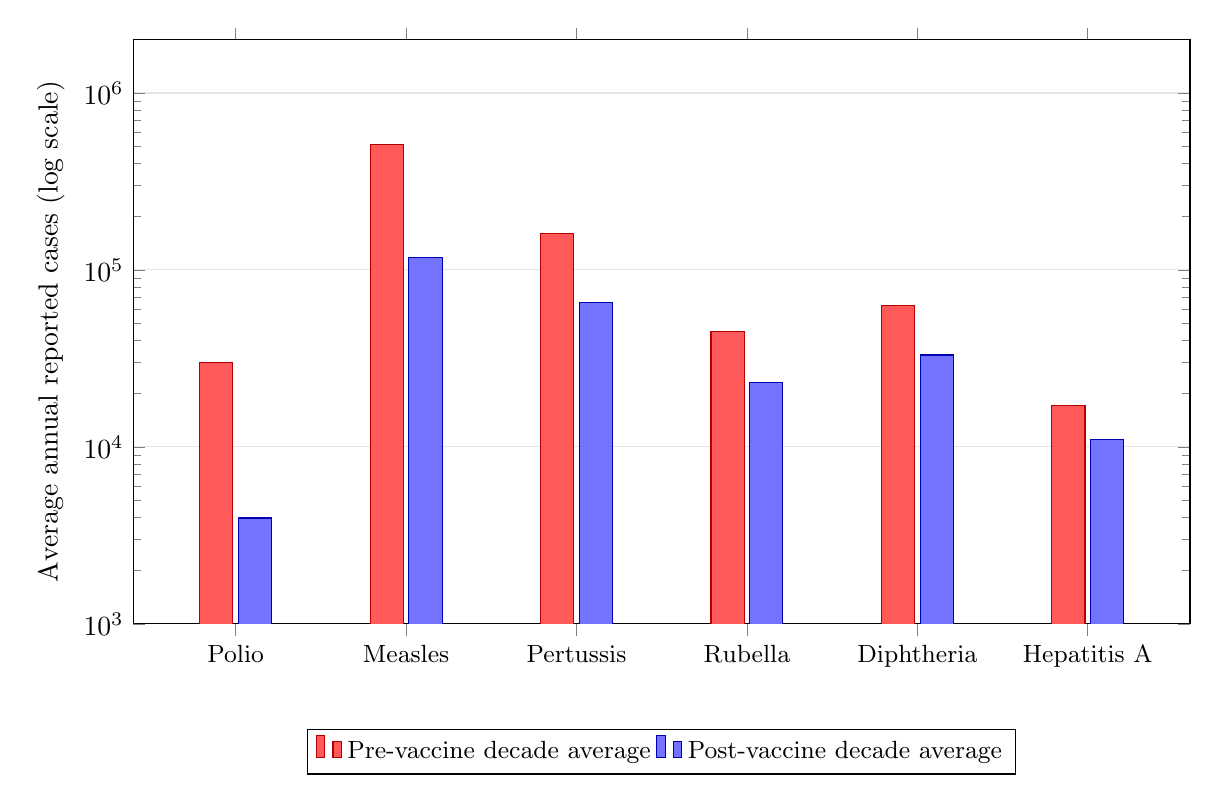
\begin{tikzpicture}
\begin{axis}[
    ybar=2pt,
    width=15cm,
    height=9cm,
    ymode=log,
    log basis y=10,
    ymin=1000,
    ymax=2000000,
    ylabel={Average annual reported cases (log scale)},
    symbolic x coords={Polio,Measles,Pertussis,Rubella,Diphtheria,Hepatitis A},
    xtick=data,
    xticklabel style={font=\small},
    bar width=12pt,
    enlarge x limits=0.12,
    legend style={at={(0.5,-0.18)}, anchor=north, legend columns=2, font=\small},
    ymajorgrids=true,
    grid style={gray!20},
    nodes near coords style={font=\scriptsize, rotate=90, anchor=west},
]
\addplot[fill=red!65, draw=red!70!black] coordinates {
    (Polio, 30093)
    (Measles, 511984)
    (Pertussis, 159976)
    (Rubella, 44997)
    (Diphtheria, 62594)
    (Hepatitis A, 17105)
};
\addplot[fill=blue!55, draw=blue!70!black] coordinates {
    (Polio, 3963)
    (Measles, 117631)
    (Pertussis, 65646)
    (Rubella, 23241)
    (Diphtheria, 33046)
    (Hepatitis A, 10989)
};
\legend{Pre-vaccine decade average, Post-vaccine decade average}
\end{axis}
\end{tikzpicture}
\caption{Average annual reported cases in the decade before (red) and the decade after (blue) each disease's vaccine introduction, plotted on a logarithmic scale so that diseases spanning four orders of magnitude in case counts can share one panel. The corresponding percentage reductions are $-86.83\%$ for polio, $-77.02\%$ for measles, $-58.97\%$ for pertussis, $-48.35\%$ for rubella, $-47.21\%$ for diphtheria, and $-35.76\%$ for hepatitis~A. Diphtheria uses the 1916--1922 pre-vaccine window because the series begins in 1916.}
\label{fig:vaccine_impact}
\end{figure}

The paired-bar form makes the absolute scale of the reduction visible in addition to its percentage. Polio drops from 30{,}093 to 3{,}963 average annual cases, a $-86.83\%$ reduction that is consistent with the rapid collapse in reported cases after the 1955 Salk vaccine. Measles drops from 511{,}984 to 117{,}631 cases ($-77.02\%$) after the 1963 live-attenuated vaccine, and pertussis from 159{,}976 to 65{,}646 ($-58.97\%$) after the 1948 DTP introduction. Rubella falls from 44{,}997 to 23{,}241 ($-48.35\%$) after the 1969 vaccine. The diphtheria entry, 62{,}594 down to 33{,}046 ($-47.21\%$), is notable because it is the only city-grain disease in the dataset and because the real Project Tycho Level 1 series includes 1916--1922 as genuine pre-vaccine years rather than requiring an imputed baseline. Hepatitis A shows the smallest reduction, from 17{,}105 to 10{,}989 ($-35.76\%$), consistent with its recent vaccine year (1995) and the more gradual rollout of routine adolescent and high-risk vaccination in the United States.

\subsection{Seasonal Patterns}

Query Q4 reveals distinct seasonal signatures for different diseases. Figure~\ref{fig:seasonal} shows average weekly reported cases by calendar month for four representative diseases, computed across the full 1916--2011 time range of the real Project Tycho Level 1 dataset.

\begin{figure}[H]
\centering
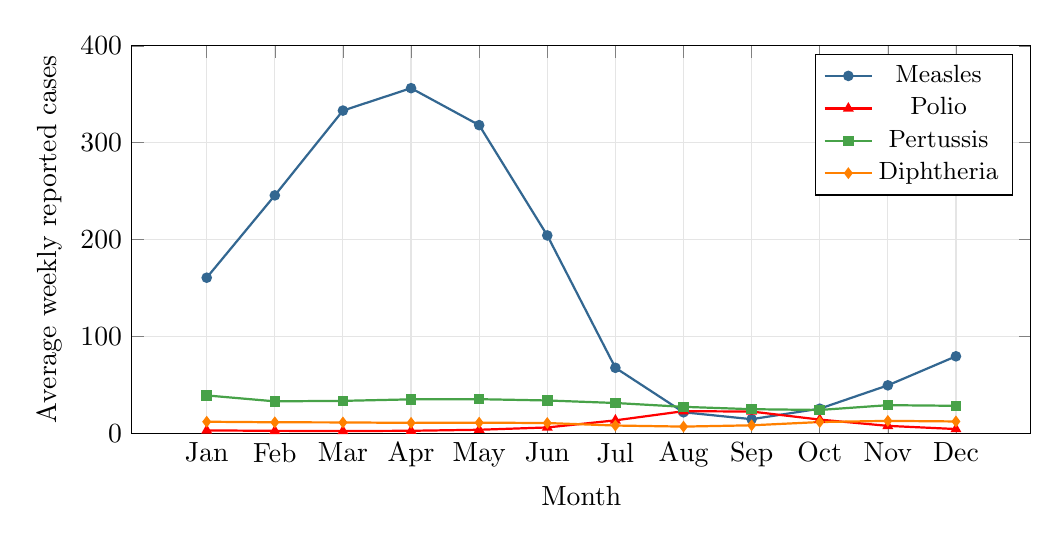
\begin{tikzpicture}
\begin{axis}[
    width=13cm,
    height=6.5cm,
    xlabel={Month},
    ylabel={Average weekly reported cases},
    xtick={1,2,...,12},
    xticklabels={Jan,Feb,Mar,Apr,May,Jun,Jul,Aug,Sep,Oct,Nov,Dec},
    legend style={at={(0.98,0.98)}, anchor=north east, font=\small},
    grid=major,
    grid style={gray!20},
    ymin=0,
    ymax=400,
]
% Measles: peaks in April (month 4)
\addplot[thick, pgblue, mark=*,mark size=1.5pt] coordinates {
    (1,160.48)(2,245.52)(3,333.09)(4,356.25)(5,318.06)(6,204.15)(7,67.44)(8,21.51)(9,14.36)(10,25.21)(11,49.31)(12,79.32)
};
% Polio: peaks in August (month 8)
\addplot[thick, red, mark=triangle*,mark size=1.5pt] coordinates {
    (1,2.77)(2,2.31)(3,2.11)(4,2.38)(5,3.43)(6,5.82)(7,13.15)(8,22.63)(9,22.25)(10,13.94)(11,7.46)(12,4.18)
};
% Pertussis: peaks in May (month 5)
\addplot[thick, mongogreen, mark=square*,mark size=1.5pt] coordinates {
    (1,38.90)(2,32.79)(3,33.29)(4,34.84)(5,35.01)(6,33.69)(7,31.08)(8,27.12)(9,24.67)(10,23.88)(11,28.84)(12,28.18)
};
% Diphtheria: peaks in Jan (month 1), CITY grain so smaller absolute values
\addplot[thick, orange, mark=diamond*,mark size=1.5pt] coordinates {
    (1,11.72)(2,11.16)(3,11.02)(4,10.55)(5,10.78)(6,10.38)(7,7.81)(8,6.70)(9,8.03)(10,11.41)(11,12.61)(12,12.01)
};
\legend{Measles, Polio, Pertussis, Diphtheria}
\end{axis}
\end{tikzpicture}
\caption{Seasonal patterns in average weekly reported cases by calendar month, computed from the real Project Tycho Level 1 dataset. Measles peaks in late winter and early spring. Polio peaks in late summer. Pertussis is broadly distributed with a spring maximum. Diphtheria (city-grain only, 1916--1947) peaks in late autumn and early winter. Values for polio and diphtheria are reported on the same axis even though their absolute rates differ substantially from the airborne childhood diseases.}
\label{fig:seasonal}
\end{figure}

The real-data seasonal signatures align with established epidemiology. Measles, an airborne respiratory virus, peaks during the cold months when indoor contact rates are highest. Polio, transmitted through the faecal-oral route, peaks in late summer when warm-weather exposure to contaminated water is most common. Pertussis is less sharply seasonal but has a spring maximum. Diphtheria's modest peak in late autumn and early winter matches the historical clinical description of the disease as most active in cooler months.

\subsection{Disease Trends by Decade}

The pivot operation (Table~\ref{tab:pivot}) provides a cross-tabulated view of total reported cases by disease and decade for the real Project Tycho Level 1 dataset. Zero values in the table indicate decades in which the disease had no reported rows at the relevant grain in the Level 1 release, not necessarily an absence of disease.

\begin{table}[H]
\centering
\caption{Total reported cases by disease and decade from the real Project Tycho Level 1 dataset (1910s--2010s). Diphtheria totals are from city-level reporting; all other diseases are from state-level reporting.}
\label{tab:pivot}
\resizebox{\textwidth}{!}{%
\begin{tabular}{rrrrrrrrr}
\toprule
\textbf{Decade} & \textbf{Measles} & \textbf{Pertussis} & \textbf{Polio} & \textbf{Diphtheria} & \textbf{Hep.~A} & \textbf{Mumps} & \textbf{Rubella} & \textbf{Smallpox} \\
\midrule
1910 &           0 &          0 &          0 &   224{,}604 &          0 &          0 &          0 &          0 \\
1920 &    822{,}398 &          0 &     7{,}502 &   523{,}007 &          0 &          0 &          0 &     74{,}859 \\
1930 &  4{,}863{,}625 &    394{,}722 &    76{,}628 &   126{,}505 &          0 &          0 &          0 &    148{,}159 \\
1940 &  4{,}706{,}673 &  1{,}348{,}766 &   164{,}093 &    27{,}124 &          0 &          0 &          0 &      9{,}733 \\
1950 &  5{,}201{,}222 &    391{,}424 &   246{,}255 &          0 &          0 &          0 &          0 &          77 \\
1960 &  2{,}645{,}923 &          0 &     6{,}331 &          0 &   161{,}912 &    224{,}117 &    187{,}738 &          0 \\
1970 &    346{,}590 &     8{,}539 &          0 &          0 &   397{,}552 &    538{,}642 &    232{,}411 &          0 \\
1980 &     50{,}495 &    23{,}360 &          0 &          0 &   190{,}957 &     52{,}693 &     11{,}500 &          0 \\
1990 &     33{,}929 &    40{,}775 &          0 &          0 &   169{,}439 &     15{,}956 &      3{,}157 &          0 \\
2000 &         143 &    96{,}222 &          0 &          0 &     51{,}340 &         702 &         160 &          0 \\
2010 &           0 &    25{,}212 &          0 &          0 &      5{,}162 &          0 &          0 &          0 \\
\bottomrule
\end{tabular}%
}
\end{table}

Several patterns are visible. Measles rises through the 1930s--1950s, peaks at over 5.2~million cases in the 1950s, and drops dramatically from the 1960s onward once the 1963 vaccine takes effect. Polio cases peak in the 1940s and collapse after 1955. Diphtheria is visible only at city grain from 1916 through 1947, after which the Level 1 dataset no longer reports it at that grain. Hepatitis A first appears in the 1960s (the year national reporting standardised) and then tracks a rise-and-decline pattern driven by the 1995 vaccine. Smallpox drops from 74{,}859 cases in the 1920s to zero after 1960, consistent with the historical elimination of endemic US transmission. The pivot also makes visible the reporting-era boundaries for several diseases, which is a real characteristic of the Tycho Level 1 release rather than an artefact of the ETL pipeline.

\subsection{Frontend Dashboard}

The React dashboard provides four pages. The Overview page displays system health, record counts, and summary charts. The OLAP Explorer allows interactive query execution against any backend with parameter configuration and chart auto-generation, and exposes the three graph-only queries (Q11--Q13) as additional Neo4j entries in the same query selector rather than on a separate page. The Comparison Dashboard runs queries across all backends and presents execution times as bar charts alongside per-backend result tables. The Live Stream page connects to the Kafka SSE endpoint and displays real-time event counts and anomaly alerts.


\begin{figure}[H]
\centering
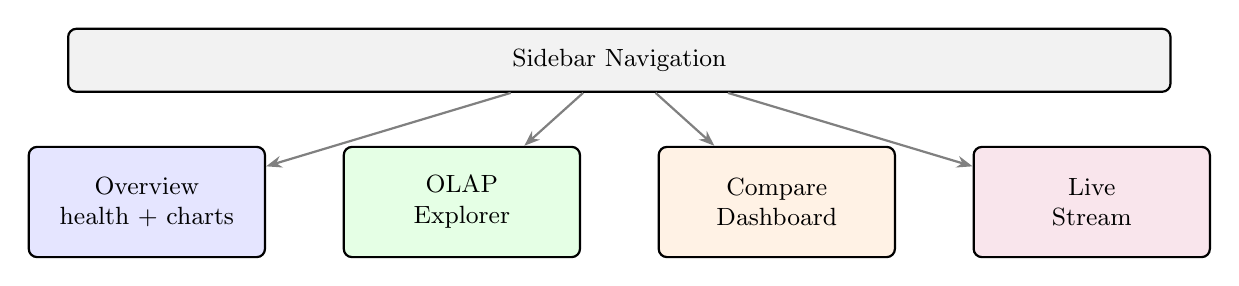
\begin{tikzpicture}[
  every node/.style={font=\small},
  page/.style={rectangle, draw, thick, rounded corners=3pt, minimum width=3cm, minimum height=1.4cm, align=center},
  arr/.style={-{Stealth[length=2mm]}, thick, gray},
]

\node[page, fill=blue!10] (home) at (0, 0) {Overview\\health + charts};
\node[page, fill=green!10] (explorer) at (4, 0) {OLAP\\Explorer};
\node[page, fill=orange!10] (compare) at (8, 0) {Compare\\Dashboard};
\node[page, fill=purple!10] (stream) at (12, 0) {Live\\Stream};

\node[rectangle, draw, thick, fill=gray!10, minimum width=14cm, minimum height=0.8cm, rounded corners=3pt] (nav) at (6, 1.8) {Sidebar Navigation};

\draw[arr] (nav) -- (home);
\draw[arr] (nav) -- (explorer);
\draw[arr] (nav) -- (compare);
\draw[arr] (nav) -- (stream);

\end{tikzpicture}
\caption{React dashboard page layout with four pages accessed through a persistent sidebar. The three graph-only queries (Q11--Q13) are surfaced as additional Neo4j entries inside the OLAP Explorer instead of on a dedicated Graph Explorer page.}
\label{fig:dashboard_layout}
\end{figure}


% ================================================================
% 7. DISCUSSION
% ================================================================
\section{Discussion}
\label{sec:discussion}

\subsection{Backend Strengths and Trade-offs}

The cross-backend comparison shows that each database paradigm excels in a different domain of analytical work.

\subsubsection{PostgreSQL}

PostgreSQL is the strongest all-round choice for structured OLAP workloads on this dataset. The star schema, combined with the query optimiser's handling of multi-way joins, produces competitive execution times across all ten standard queries against the real Project Tycho Level 1 data. Window functions (\texttt{LAG}, \texttt{RANK}, \texttt{STDDEV}) and aggregate correlation (\texttt{CORR}) are native language features that execute in a single pass. \texttt{LATERAL} joins allow the vaccination impact query (Q8) to compute per-disease pre/post comparisons without procedural loops. The four materialised views remove repeated aggregation work for common access patterns. PostgreSQL's main limitation is its lack of variable-length relationship support. Simulating the state border adjacency graph in SQL would require a self-join table and recursive CTEs, which are syntactically awkward and computationally expensive for multi-hop traversals.

\subsubsection{MongoDB}

MongoDB is most competitive on queries that benefit from selective filtering against its denormalised document structure. On Q2 and Q3 MongoDB outperforms PostgreSQL because the compound index allows direct document retrieval without any joins. The dimension attributes embedded in each document mean that a single index seek resolves the entire query. The \texttt{\$setWindowFields} stage (available since MongoDB 5.0 and retained in MongoDB 8) brings window function capabilities into the aggregation pipeline, enabling the year-over-year calculation in Q5. For broad aggregation queries (Q1, Q6, Q9), MongoDB is slower than PostgreSQL on the same benchmark, reflecting the overhead of processing bucket documents through multi-stage pipelines compared to PostgreSQL's scan of pre-joined fact rows with a single composite index.

The main limitation of MongoDB's approach is visible in Q6, where the lack of a native correlation function prevents a direct equivalent of PostgreSQL's \texttt{CORR} aggregate. The implementation uses a simplified per-disease co-occurrence count that answers a related but different question. The broader pattern is that MongoDB's aggregation framework is strong for straightforward group-by operations and becomes less ergonomic when the analysis requires cross-group statistical comparisons.

\subsubsection{Neo4j}

Neo4j is the slowest backend on all ten standard OLAP queries, which is expected and not the appropriate lens through which to evaluate a graph database. Neo4j's value lies in its three exclusive queries. Q11 traces disease spread through border adjacency relationships, finding temporal lags between neighbouring states that suggest geographic transmission patterns. Q12 computes per-state disease composition profiles through a single traversal. Q13 measures geographic coverage through distinct state-year counting across the graph. These queries would require either recursive CTEs or application-level computation in the other backends.

The performance gap between Neo4j and the other backends on standard OLAP queries stems from the multi-hop traversal required by the time hierarchy. Every query must traverse Month $\rightarrow$ Quarter $\rightarrow$ Year $\rightarrow$ Decade to reach a year or decade value, which adds constant overhead per aggregate node. A flatter graph model with denormalised time properties on the MonthlyAggregate nodes would reduce this overhead at the cost of losing the hierarchical drill-down capability.

\subsection{Data Modeling Implications}

The three data models represent fundamentally different trade-offs between normalization, redundancy, and query flexibility.

The star schema's normalised dimensions provide referential integrity and compact storage but require joins for every query. This trade-off favours queries that aggregate across large portions of the fact table, where the join cost is amortised over many rows.

The Bucket Pattern's embedded documents duplicate dimension data across 155{,}063 bucket documents but remove join overhead entirely. This trade-off favours selective queries that touch a small fraction of the collection. The cost is higher per-row storage and the need to keep embedded data consistent if dimension values change, which is not a concern for this historical dataset. On the real dataset the MongoDB collection is 114~MB compared to 92~MB for PostgreSQL, a 24\% storage premium for the join-free document layout.

The graph model's relationship-first approach introduces the highest node count (619{,}646 nodes across Observation, MonthlyAggregate, and dimension/hierarchy nodes) and 1{,}845{,}584 relationships. Its on-disk store of 103~MB sits between PostgreSQL's 92~MB star schema and MongoDB's 114~MB bucket collection, because the relationship store alone accounts for 64~MB of the total even though each edge is a compact fixed-width record. The cost of the relationship-heavy layout is also visible at query time, since every Neo4j row in Table~\ref{tab:query_perf} pays a multi-hop traversal penalty on standard aggregation queries that do not benefit from graph traversal.

\subsection{Limitations}

All timings in Section~\ref{sec:results} are measured through the FastAPI \texttt{/api/v1/query} endpoint running inside the Docker Compose stack on the real Project Tycho Level 1 load, with seven consecutive runs against a warm cache and the first two runs dropped as warmup. The backend container, the three database containers and the benchmark client share the same Docker bridge network, so the reported milliseconds include Python driver overhead and container-to-container socket latency. They are therefore comparable across the three backends within a single row of Table~\ref{tab:query_perf} but should not be read as absolute figures for a native (non-containerised) deployment, where driver and network overhead would be lower for all three systems.

Real Project Tycho Level 1 reporting is uneven across the eight diseases and across time. Diphtheria is reported only at city level for the years 1916--1947. National mumps surveillance began only in 1968. Hepatitis A reporting standardised in the 1960s. The pivot table reflects these reporting boundaries rather than hiding them, and the vaccine impact analysis omits diseases for which the dataset does not cover the appropriate pre-vaccine window. These reporting characteristics are properties of the source data, not of the warehouse, and they limit any cross-disease comparison that assumes uniform reporting coverage.


% ================================================================
% 8. CONCLUSION
% ================================================================
\section{Conclusion}
\label{sec:conclusion}

This project shows that a single real epidemiological dataset, Project Tycho Level 1 with its 473{,}189 cleaned weekly observations across 1916--2011, can be modelled in three fundamentally different database paradigms with distinct strengths. PostgreSQL with a Kimball star schema is the most capable and efficient platform for structured OLAP analytics, providing the broadest query expressiveness and strong overall performance. MongoDB with the Bucket Pattern offers competitive performance for filtered, selective queries and removes join overhead through denormalisation. Neo4j provides unique analytical capabilities through graph traversal, particularly for geographic spread analysis over state border relationships and for the city-to-state hierarchy required by the diphtheria portion of the dataset.

The unified API and comparison engine provide a practical means to evaluate these trade-offs empirically. By executing the same logical query across all three backends concurrently and returning the native query text alongside results and timing, the system supports direct comparison of performance, query complexity, and expressiveness.

The streaming layer shows how Kafka and ksqlDB can extend a batch-oriented warehouse with event processing. The four-stage ksqlDB pipeline (ingest, validate, aggregate, alert) runs as persistent queries that process events as they arrive, providing continuous monitoring without polling.

Possible extensions include adding time-series database backends (for example TimescaleDB, InfluxDB) for additional comparison against the three systems already benchmarked, implementing incremental ETL loads rather than full refreshes, extending the graph model with richer geographic and demographic relationships to enable additional graph-specific analyses beyond Q11--Q13, and scaling the measurement protocol to larger synthetic loads in order to characterise how the relative performance of PostgreSQL, MongoDB, and Neo4j evolves beyond the 473{,}189-row working set.

% ================================================================
% REFERENCES
% ================================================================
\newpage
\begin{thebibliography}{99}
\setlength{\itemsep}{4pt}

\bibitem{vanpanhuis2013}
W.~G. van~Panhuis, J.~Grefenstette, S.~Y. Jung, N.~S. Chok, A.~Cross, H.~Burke, et~al., ``Contagious diseases in the United States from 1888 to the present,'' \textit{New England Journal of Medicine}, vol.~369, no.~22, pp.~2152--2158, 2013.

\bibitem{vanpanhuis2018}
W.~G. van~Panhuis, A.~Cross, and D.~S. Burke, ``Project Tycho 2.0: a repository to improve the integration and reuse of data for global population health,'' \textit{Journal of the American Medical Informatics Association}, vol.~25, no.~12, pp.~1608--1616, 2018.

\bibitem{kimball2013}
R.~Kimball and M.~Ross, \textit{The Data Warehouse Toolkit: The Definitive Guide to Dimensional Modeling}, 3rd~ed. Indianapolis, IN: John Wiley \& Sons, 2013.

\bibitem{inmon2005}
W.~H. Inmon, \textit{Building the Data Warehouse}, 4th~ed. Indianapolis, IN: John Wiley \& Sons, 2005.

\bibitem{codd1993}
E.~F. Codd, S.~B. Codd, and C.~T. Salley, ``Providing OLAP to user-analysts: An IT mandate,'' Codd and Date, Inc., Tech.~Rep., 1993.

\bibitem{chaudhuri1997}
S.~Chaudhuri and U.~Dayal, ``An overview of data warehousing and OLAP technology,'' \textit{ACM SIGMOD Record}, vol.~26, no.~1, pp.~65--74, 1997.

\bibitem{copeland2012}
R.~Copeland, \textit{MongoDB Applied Design Patterns}. Sebastopol, CA: O'Reilly Media, 2013.

\bibitem{robinson2015}
I.~Robinson, J.~Webber, and E.~Eifrem, \textit{Graph Databases: New Opportunities for Connected Data}, 2nd~ed. Sebastopol, CA: O'Reilly Media, 2015.

\bibitem{angles2008}
R.~Angles and C.~Gutierrez, ``Survey of graph database models,'' \textit{ACM Computing Surveys}, vol.~40, no.~1, pp.~1--39, 2008.

\bibitem{kreps2011}
J.~Kreps, N.~Narkhede, and J.~Rao, ``Kafka: A distributed messaging system for log processing,'' in \textit{Proc. NetDB Workshop}, Athens, Greece, 2011, pp.~1--7.

\bibitem{kafkadocs}
Apache Software Foundation, ``Apache Kafka Documentation,'' 2026. [Online]. Available: \url{https://kafka.apache.org/documentation/}

\bibitem{ksqldocs}
Confluent, Inc., ``ksqlDB Documentation,'' 2026. [Online]. Available: \url{https://docs.ksqldb.io/en/latest/}

\bibitem{pgdocs}
PostgreSQL Global Development Group, ``PostgreSQL 18 Documentation,'' 2026. [Online]. Available: \url{https://www.postgresql.org/docs/18/}

\bibitem{mongodocs}
MongoDB, Inc., ``MongoDB 8.0 Manual,'' 2026. [Online]. Available: \url{https://www.mongodb.com/docs/v8.0/}

\bibitem{neo4jdocs}
Neo4j, Inc., ``Neo4j 2026.03 Documentation,'' 2026. [Online]. Available: \url{https://neo4j.com/docs/operations-manual/current/}

\bibitem{tychoportal}
University of Pittsburgh, ``Project Tycho: Data for Health,'' 2026. [Online]. Available: \url{https://www.tycho.pitt.edu/}

\end{thebibliography}


% ================================================================
% APPENDIX
% ================================================================
\newpage
\section*{Appendix}
\addcontentsline{toc}{section}{Appendix}
\appendix
\section{Query Implementations in All Three Backends}
\label{app:queries}

This appendix contains the complete implementations of all thirteen decision support queries. For the ten cross-backend queries (Q1--Q10), the PostgreSQL, MongoDB, and Neo4j versions are shown side by side so that the reader can see how the same analytical intent is expressed in SQL, the MongoDB aggregation framework, and Cypher. Queries Q11--Q13 are shown for Neo4j only, since they depend on the \texttt{BORDERS} relationship that does not exist in the other two backends. The code listings are taken directly from \texttt{backend/app/services/postgres\_service.py}, \texttt{mongo\_service.py}, and \texttt{neo4j\_service.py}; minor whitespace and inline comment adjustments have been applied for readability.

\lstset{basicstyle=\ttfamily\footnotesize}

\subsection*{Q1: Total Cases by Disease and Decade (Roll-up)}

\begin{lstlisting}[language=SQL, caption={Q1: PostgreSQL.}]
SELECT d.disease_name, t.decade,
       SUM(f.case_count) AS total_cases,
       ROUND(AVG(f.incidence_rate)::numeric, 2) AS avg_incidence
FROM   fact_disease_incidence f
JOIN   dim_disease  d ON f.disease_key  = d.disease_key
JOIN   dim_time     t ON f.time_key     = t.time_key
JOIN   dim_location l ON f.location_key = l.location_key
WHERE  l.loc_type = 'STATE'
GROUP BY d.disease_name, t.decade
ORDER BY d.disease_name, t.decade;
\end{lstlisting}

\begin{lstlisting}[language={}, caption={Q1: MongoDB.}]
db.disease_observations.aggregate([
  { "$group": {
      "_id": { "disease": "$disease.name",
               "decade":  "$time_bucket.decade" },
      "total_cases":   { "$sum": "$monthly_summary.total_cases" },
      "avg_incidence": { "$avg": "$monthly_summary.avg_incidence_rate" }
  }},
  { "$sort": { "_id.disease": 1, "_id.decade": 1 } },
  { "$project": { "_id": 0, "disease_name": "$_id.disease",
                  "decade": "$_id.decade", "total_cases": 1,
                  "avg_incidence": { "$round": ["$avg_incidence", 2] } } }
])
\end{lstlisting}

\begin{lstlisting}[language=cypher, caption={Q1: Neo4j.}]
MATCH (a:MonthlyAggregate)-[:SUMMARIZES_DISEASE]->(d:Disease),
      (a)-[:SUMMARIZES_MONTH]->(m:Month)-[:IN_QUARTER]->(:Quarter)
      -[:IN_YEAR]->(y:Year)-[:IN_DECADE]->(dec:Decade)
RETURN d.name AS disease_name, dec.decade AS decade,
       SUM(a.total_cases) AS total_cases,
       ROUND(AVG(a.avg_incidence), 2) AS avg_incidence
ORDER BY d.name, dec.decade;
\end{lstlisting}


\subsection*{Q2: Measles Incidence by State for a Specific Year (Slice)}

\begin{lstlisting}[language=SQL, caption={Q2: PostgreSQL.}]
SELECT l.state_name, SUM(f.case_count) AS total_cases,
       ROUND(AVG(f.incidence_rate)::numeric, 2) AS avg_incidence
FROM   fact_disease_incidence f
JOIN   dim_disease  d ON f.disease_key  = d.disease_key
JOIN   dim_time     t ON f.time_key     = t.time_key
JOIN   dim_location l ON f.location_key = l.location_key
WHERE  d.disease_name = 'MEASLES'
  AND  t.year = %s
  AND  l.loc_type = 'STATE'
GROUP BY l.state_name
ORDER BY total_cases DESC;
\end{lstlisting}

\begin{lstlisting}[language={}, caption={Q2: MongoDB.}]
db.disease_observations.aggregate([
  { "$match": { "disease.name": "MEASLES", "time_bucket.year": year } },
  { "$group": { "_id": "$location.state_name",
                "total_cases":   { "$sum": "$monthly_summary.total_cases" },
                "avg_incidence": { "$avg": "$monthly_summary.avg_incidence_rate" } } },
  { "$sort": { "total_cases": -1 } },
  { "$project": { "_id": 0, "state_name": "$_id", "total_cases": 1,
                  "avg_incidence": { "$round": ["$avg_incidence", 2] } } }
])
\end{lstlisting}

\begin{lstlisting}[language=cypher, caption={Q2: Neo4j.}]
MATCH (a:MonthlyAggregate)-[:SUMMARIZES_DISEASE]->(d:Disease {name:'MEASLES'}),
      (a)-[:SUMMARIZES_STATE]->(s:State),
      (a)-[:SUMMARIZES_MONTH]->(m:Month)-[:IN_QUARTER]->(:Quarter)
      -[:IN_YEAR]->(y:Year {year: $year})
RETURN s.name AS state_name, SUM(a.total_cases) AS total_cases,
       ROUND(AVG(a.avg_incidence), 2) AS avg_incidence
ORDER BY total_cases DESC;
\end{lstlisting}


\subsection*{Q3: Top 10 States for Disease and Year Range (Dice)}

\begin{lstlisting}[language=SQL, caption={Q3: PostgreSQL.}]
SELECT l.state_name, SUM(f.case_count) AS total_cases
FROM   fact_disease_incidence f
JOIN   dim_disease  d ON f.disease_key  = d.disease_key
JOIN   dim_time     t ON f.time_key     = t.time_key
JOIN   dim_location l ON f.location_key = l.location_key
WHERE  d.disease_name = %s
  AND  t.year BETWEEN %s AND %s
  AND  l.loc_type = 'STATE'
GROUP BY l.state_name
ORDER BY total_cases DESC
LIMIT  10;
\end{lstlisting}

\begin{lstlisting}[language={}, caption={Q3: MongoDB.}]
db.disease_observations.aggregate([
  { "$match": { "disease.name": disease,
                "time_bucket.year": { "$gte": start_year, "$lte": end_year } } },
  { "$group": { "_id": "$location.state_name",
                "total_cases": { "$sum": "$monthly_summary.total_cases" } } },
  { "$sort":   { "total_cases": -1 } },
  { "$limit":  10 },
  { "$project": { "_id": 0, "state_name": "$_id", "total_cases": 1 } }
])
\end{lstlisting}

\begin{lstlisting}[language=cypher, caption={Q3: Neo4j.}]
MATCH (a:MonthlyAggregate)-[:SUMMARIZES_DISEASE]->(d:Disease {name: $disease}),
      (a)-[:SUMMARIZES_STATE]->(s:State),
      (a)-[:SUMMARIZES_MONTH]->(m:Month)-[:IN_QUARTER]->(:Quarter)
      -[:IN_YEAR]->(y:Year)
WHERE y.year >= $startYear AND y.year <= $endYear
RETURN s.name AS state_name, SUM(a.total_cases) AS total_cases
ORDER BY total_cases DESC
LIMIT 10;
\end{lstlisting}


\subsection*{Q4: Seasonal Pattern: Average Weekly Cases per Month}

\begin{lstlisting}[language=SQL, caption={Q4: PostgreSQL.}]
SELECT t.month, t.month_name,
       ROUND(AVG(f.case_count)::numeric, 2) AS avg_weekly_cases
FROM   fact_disease_incidence f
JOIN   dim_disease  d ON f.disease_key  = d.disease_key
JOIN   dim_time     t ON f.time_key     = t.time_key
JOIN   dim_location l ON f.location_key = l.location_key
WHERE  d.disease_name = %s AND l.loc_type = 'STATE'
GROUP BY t.month, t.month_name
ORDER BY t.month;
\end{lstlisting}

\begin{lstlisting}[language={}, caption={Q4: MongoDB. \texttt{\$unwind} exposes individual weekly observations for averaging.}]
db.disease_observations.aggregate([
  { "$match":  { "disease.name": disease } },
  { "$unwind": "$weekly_observations" },
  { "$group":  { "_id": { "month": "$time_bucket.month",
                          "month_name": "$time_bucket.month_name" },
                 "avg_weekly_cases": { "$avg": "$weekly_observations.cases" } } },
  { "$sort":   { "_id.month": 1 } },
  { "$project": { "_id": 0, "month": "$_id.month",
                  "month_name": "$_id.month_name",
                  "avg_weekly_cases": { "$round": ["$avg_weekly_cases", 2] } } }
])
\end{lstlisting}

\begin{lstlisting}[language=cypher, caption={Q4: Neo4j.}]
MATCH (a:MonthlyAggregate)-[:SUMMARIZES_DISEASE]->(d:Disease {name: $disease}),
      (a)-[:SUMMARIZES_MONTH]->(m:Month)
RETURN m.month AS month, m.month_name AS month_name,
       ROUND(AVG(a.total_cases /
             CASE WHEN a.observation_count = 0 THEN 1
                  ELSE a.observation_count END), 2) AS avg_weekly_cases
ORDER BY m.month;
\end{lstlisting}


\subsection*{Q5: Year-over-Year Change in Cases per State}

\begin{lstlisting}[language=SQL, caption={Q5: PostgreSQL. \texttt{LAG()} provides the previous year's value in-place.}]
WITH yearly AS (
  SELECT d.disease_name, l.state_name, t.year,
         SUM(f.case_count) AS total_cases
  FROM   fact_disease_incidence f
  JOIN   dim_disease  d ON f.disease_key  = d.disease_key
  JOIN   dim_time     t ON f.time_key     = t.time_key
  JOIN   dim_location l ON f.location_key = l.location_key
  WHERE  d.disease_name = %s AND l.loc_type = 'STATE'
  GROUP BY d.disease_name, l.state_name, t.year
)
SELECT state_name, year, total_cases,
       LAG(total_cases) OVER (PARTITION BY state_name ORDER BY year)
         AS prev_year_cases,
       ROUND(((total_cases - LAG(total_cases) OVER
               (PARTITION BY state_name ORDER BY year))::numeric
         / NULLIF(LAG(total_cases) OVER
               (PARTITION BY state_name ORDER BY year), 0)) * 100, 2)
         AS yoy_pct_change
FROM yearly
ORDER BY state_name, year;
\end{lstlisting}

\begin{lstlisting}[language={}, caption={Q5: MongoDB. \texttt{\$setWindowFields} with \texttt{\$shift} supplies the previous row.}]
db.disease_observations.aggregate([
  { "$match": { "disease.name": disease } },
  { "$group": { "_id": { "state": "$location.state_name",
                         "year":  "$time_bucket.year" },
                "total_cases": { "$sum": "$monthly_summary.total_cases" } } },
  { "$sort": { "_id.state": 1, "_id.year": 1 } },
  { "$setWindowFields": {
      "partitionBy": "$_id.state",
      "sortBy": { "_id.year": 1 },
      "output": { "prev_year_cases":
                  { "$shift": { "output": "$total_cases", "by": -1 } } } } },
  { "$addFields": { "yoy_pct_change": {
      "$cond": { "if": { "$and": [
                           { "$ne": ["$prev_year_cases", null] },
                           { "$ne": ["$prev_year_cases", 0] } ] },
                 "then": { "$round": [ { "$multiply": [
                             { "$divide": [
                                { "$subtract": ["$total_cases",
                                                "$prev_year_cases"] },
                                "$prev_year_cases" ] },
                             100 ] }, 2 ] },
                 "else": null } } } },
  { "$project": { "_id": 0, "state_name": "$_id.state",
                  "year": "$_id.year", "total_cases": 1,
                  "prev_year_cases": 1, "yoy_pct_change": 1 } }
])
\end{lstlisting}

\begin{lstlisting}[language=cypher, caption={Q5: Neo4j. \texttt{COLLECT} + \texttt{UNWIND RANGE} emulates the row-to-row comparison.}]
MATCH (a:MonthlyAggregate)-[:SUMMARIZES_DISEASE]->(d:Disease {name: $disease}),
      (a)-[:SUMMARIZES_STATE]->(s:State),
      (a)-[:SUMMARIZES_MONTH]->(m:Month)-[:IN_QUARTER]->(:Quarter)
      -[:IN_YEAR]->(y:Year)
WITH s.name AS state, y.year AS year, SUM(a.total_cases) AS total_cases
ORDER BY state, year
WITH state, COLLECT({year: year, cases: total_cases}) AS yearly_data
UNWIND RANGE(1, SIZE(yearly_data)-1) AS i
WITH state, yearly_data[i] AS curr, yearly_data[i-1] AS prev
RETURN state AS state_name, curr.year AS year, curr.cases AS total_cases,
       prev.cases AS prev_year_cases,
       ROUND(toFloat(curr.cases - prev.cases) /
             CASE WHEN prev.cases = 0 THEN 1 ELSE prev.cases END * 100, 2)
             AS yoy_pct_change
ORDER BY state, year;
\end{lstlisting}


\subsection*{Q6: Disease Co-occurrence by State and Year}

\begin{lstlisting}[language=SQL, caption={Q6: PostgreSQL. \texttt{CORR()} computes a Pearson correlation of yearly state totals for every disease pair.}]
WITH state_year_disease AS (
  SELECT l.state_name, t.year, d.disease_name,
         SUM(f.case_count) AS total_cases
  FROM   fact_disease_incidence f
  JOIN   dim_disease  d ON f.disease_key  = d.disease_key
  JOIN   dim_time     t ON f.time_key     = t.time_key
  JOIN   dim_location l ON f.location_key = l.location_key
  WHERE  l.loc_type = 'STATE'
  GROUP BY l.state_name, t.year, d.disease_name
  HAVING SUM(f.case_count) > 100
)
SELECT a.disease_name AS disease_a, b.disease_name AS disease_b,
       COUNT(*) AS co_occurrence_count,
       ROUND(CORR(a.total_cases, b.total_cases)::numeric, 3) AS correlation
FROM   state_year_disease a
JOIN   state_year_disease b
       ON a.state_name = b.state_name
      AND a.year       = b.year
      AND a.disease_name < b.disease_name
GROUP BY a.disease_name, b.disease_name
HAVING COUNT(*) > 10
ORDER BY correlation DESC;
\end{lstlisting}

\begin{lstlisting}[language={}, caption={Q6: MongoDB. Simplified: per-disease co-occurrence count in state-years that contain at least two diseases. The aggregation framework lacks a native correlation operator.}]
db.disease_observations.aggregate([
  { "$group": { "_id": { "state":   "$location.state_code",
                         "year":    "$time_bucket.year",
                         "disease": "$disease.name" },
                "total_cases": { "$sum": "$monthly_summary.total_cases" } } },
  { "$match": { "total_cases": { "$gt": 100 } } },
  { "$group": { "_id": { "state": "$_id.state", "year": "$_id.year" },
                "diseases": { "$addToSet": "$_id.disease" },
                "count":    { "$sum": 1 } } },
  { "$match":  { "count": { "$gte": 2 } } },
  { "$unwind": "$diseases" },
  { "$group":  { "_id": "$diseases",
                 "co_occurrence_count": { "$sum": 1 } } },
  { "$sort":   { "co_occurrence_count": -1 } },
  { "$project": { "_id": 0, "disease_a": "$_id", "co_occurrence_count": 1 } }
])
\end{lstlisting}

\begin{lstlisting}[language=cypher, caption={Q6: Neo4j. Pair enumeration via double \texttt{UNWIND} over the collected disease list.}]
MATCH (a:MonthlyAggregate)-[:SUMMARIZES_DISEASE]->(d:Disease),
      (a)-[:SUMMARIZES_STATE]->(s:State),
      (a)-[:SUMMARIZES_MONTH]->(m:Month)-[:IN_QUARTER]->(:Quarter)
      -[:IN_YEAR]->(y:Year)
WITH d.name AS disease, s.code AS state, y.year AS year,
     SUM(a.total_cases) AS total
WHERE total > 100
WITH state, year, COLLECT(disease) AS diseases
WHERE SIZE(diseases) >= 2
UNWIND diseases AS d1
UNWIND diseases AS d2
WITH d1 AS disease_a, d2 AS disease_b
WHERE disease_a < disease_b
RETURN disease_a, disease_b, COUNT(*) AS co_occurrence_count
ORDER BY co_occurrence_count DESC
LIMIT 20;
\end{lstlisting}


\subsection*{Q7: Geographic Spread: Rank States by First Report}

\begin{lstlisting}[language=SQL, caption={Q7: PostgreSQL.}]
SELECT l.state_name, MIN(t.year) AS first_reported_year,
       RANK() OVER (ORDER BY MIN(t.year)) AS spread_rank
FROM   fact_disease_incidence f
JOIN   dim_disease  d ON f.disease_key  = d.disease_key
JOIN   dim_time     t ON f.time_key     = t.time_key
JOIN   dim_location l ON f.location_key = l.location_key
WHERE  d.disease_name = %s
  AND  f.case_count > 0
  AND  l.loc_type = 'STATE'
GROUP BY l.state_name
ORDER BY first_reported_year;
\end{lstlisting}

\begin{lstlisting}[language={}, caption={Q7: MongoDB. The spread rank is computed by re-collecting the sorted result into an array and exposing \texttt{includeArrayIndex}.}]
db.disease_observations.aggregate([
  { "$match": { "disease.name": disease,
                "monthly_summary.total_cases": { "$gt": 0 } } },
  { "$group": { "_id": "$location.state_name",
                "first_reported_year": { "$min": "$time_bucket.year" } } },
  { "$sort":  { "first_reported_year": 1 } },
  { "$group": { "_id": null,
                "states": { "$push": { "state_name": "$_id",
                                       "first_reported_year":
                                         "$first_reported_year" } } } },
  { "$unwind": { "path": "$states", "includeArrayIndex": "rank" } },
  { "$project": { "_id": 0,
                  "state_name":          "$states.state_name",
                  "first_reported_year": "$states.first_reported_year",
                  "spread_rank":         { "$add": ["$rank", 1] } } }
])
\end{lstlisting}

\begin{lstlisting}[language=cypher, caption={Q7: Neo4j.}]
MATCH (a:MonthlyAggregate)-[:SUMMARIZES_DISEASE]->(d:Disease {name: $disease}),
      (a)-[:SUMMARIZES_STATE]->(s:State),
      (a)-[:SUMMARIZES_MONTH]->(m:Month)-[:IN_QUARTER]->(:Quarter)
      -[:IN_YEAR]->(y:Year)
WHERE a.total_cases > 0
WITH s.name AS state_name, MIN(y.year) AS first_reported_year
RETURN state_name, first_reported_year
ORDER BY first_reported_year;
\end{lstlisting}


\subsection*{Q8: Vaccination Impact (Pre vs.\ Post Introduction)}

\begin{lstlisting}[language=SQL, caption={Q8: PostgreSQL. A pair of \texttt{LATERAL} sub-queries pairs each disease with its pre- and post-vaccine yearly averages.}]
SELECT d.disease_name, d.vaccine_intro_year,
       pre.avg_cases  AS pre_vaccine_avg_annual_cases,
       post.avg_cases AS post_vaccine_avg_annual_cases,
       ROUND(((post.avg_cases - pre.avg_cases)::numeric
              / NULLIF(pre.avg_cases, 0)) * 100, 2) AS pct_change
FROM   dim_disease d
JOIN LATERAL (
  SELECT AVG(yearly_total)::numeric AS avg_cases FROM (
    SELECT t.year, SUM(f.case_count) AS yearly_total
    FROM   fact_disease_incidence f
    JOIN   dim_time     t ON f.time_key     = t.time_key
    JOIN   dim_location l ON f.location_key = l.location_key
    WHERE  f.disease_key = d.disease_key AND l.loc_type = 'STATE'
      AND  t.year BETWEEN d.vaccine_intro_year - 10
                      AND d.vaccine_intro_year - 1
    GROUP BY t.year ) sub
) pre ON true
JOIN LATERAL (
  SELECT AVG(yearly_total)::numeric AS avg_cases FROM (
    SELECT t.year, SUM(f.case_count) AS yearly_total
    FROM   fact_disease_incidence f
    JOIN   dim_time     t ON f.time_key     = t.time_key
    JOIN   dim_location l ON f.location_key = l.location_key
    WHERE  f.disease_key = d.disease_key AND l.loc_type = 'STATE'
      AND  t.year BETWEEN d.vaccine_intro_year + 1
                      AND d.vaccine_intro_year + 10
    GROUP BY t.year ) sub
) post ON true
WHERE  d.vaccine_intro_year IS NOT NULL
ORDER BY pct_change;
\end{lstlisting}

\begin{lstlisting}[language=Python, caption={Q8: MongoDB (Python driver). Separate pre- and post-vaccine aggregations per disease, joined in the application layer. This is why the per-backend timing reported for Q8 is not directly comparable to the other queries.}]
for d in diseases:
    name, vy = d["_id"]["name"], d["_id"]["vaccine_year"]
    if vy is None or vy < 1900: continue
    pre = list(db.disease_observations.aggregate([
        { "$match": { "disease.name": name,
                      "time_bucket.year": { "$gte": vy - 10, "$lt": vy } } },
        { "$group": { "_id": "$time_bucket.year",
                      "yearly_total": { "$sum": "$monthly_summary.total_cases" } } },
        { "$group": { "_id": None, "avg_cases": { "$avg": "$yearly_total" } } }
    ]))
    post = list(db.disease_observations.aggregate([
        { "$match": { "disease.name": name,
                      "time_bucket.year": { "$gt": vy, "$lte": vy + 10 } } },
        { "$group": { "_id": "$time_bucket.year",
                      "yearly_total": { "$sum": "$monthly_summary.total_cases" } } },
        { "$group": { "_id": None, "avg_cases": { "$avg": "$yearly_total" } } }
    ]))
    pre_avg  = pre[0]["avg_cases"]  if pre  else 0
    post_avg = post[0]["avg_cases"] if post else 0
    pct = round((post_avg - pre_avg) / pre_avg * 100, 2) if pre_avg else 0
\end{lstlisting}

\begin{lstlisting}[language=cypher, caption={Q8: Neo4j. Two \texttt{CALL} subqueries scoped to each disease compute the pre- and post-vaccine averages in a single statement.}]
MATCH (d:Disease)
WHERE d.vaccine_year IS NOT NULL AND d.vaccine_year >= 1900
CALL (d) {
  MATCH (a:MonthlyAggregate)-[:SUMMARIZES_DISEASE]->(d),
        (a)-[:SUMMARIZES_MONTH]->(m:Month)-[:IN_QUARTER]->(:Quarter)
        -[:IN_YEAR]->(y:Year)
  WHERE y.year >= d.vaccine_year - 10 AND y.year <  d.vaccine_year
  WITH y.year AS year, SUM(a.total_cases) AS yearly_total
  RETURN AVG(yearly_total) AS pre_avg
}
CALL (d) {
  MATCH (a:MonthlyAggregate)-[:SUMMARIZES_DISEASE]->(d),
        (a)-[:SUMMARIZES_MONTH]->(m:Month)-[:IN_QUARTER]->(:Quarter)
        -[:IN_YEAR]->(y:Year)
  WHERE y.year >  d.vaccine_year AND y.year <= d.vaccine_year + 10
  WITH y.year AS year, SUM(a.total_cases) AS yearly_total
  RETURN AVG(yearly_total) AS post_avg
}
RETURN d.name AS disease_name, d.vaccine_year AS vaccine_intro_year,
       ROUND(pre_avg)  AS pre_vaccine_avg_annual_cases,
       ROUND(post_avg) AS post_vaccine_avg_annual_cases,
       ROUND((post_avg - pre_avg) /
             CASE WHEN pre_avg = 0 THEN 1 ELSE pre_avg END * 100, 2)
             AS pct_change
ORDER BY pct_change;
\end{lstlisting}


\subsection*{Q9: Anomaly Detection: States Exceeding 2 Std.\ Dev.\ Above the National Mean}

\begin{lstlisting}[language=SQL, caption={Q9: PostgreSQL. A CTE pair computes per-state yearly totals and per-year national mean/stddev, then joins them to derive the z-score.}]
WITH national_stats AS (
  SELECT disease_name, year,
         AVG(state_total)    AS national_mean,
         STDDEV(state_total) AS national_stddev
  FROM (
    SELECT d.disease_name, l.state_name, t.year,
           SUM(f.case_count) AS state_total
    FROM   fact_disease_incidence f
    JOIN   dim_disease  d ON f.disease_key  = d.disease_key
    JOIN   dim_time     t ON f.time_key     = t.time_key
    JOIN   dim_location l ON f.location_key = l.location_key
    WHERE  l.loc_type = 'STATE'
    GROUP BY d.disease_name, l.state_name, t.year
  ) sub
  GROUP BY disease_name, year
),
state_totals AS (
  SELECT d.disease_name, l.state_name, t.year,
         SUM(f.case_count) AS state_total
  FROM   fact_disease_incidence f
  JOIN   dim_disease  d ON f.disease_key  = d.disease_key
  JOIN   dim_time     t ON f.time_key     = t.time_key
  JOIN   dim_location l ON f.location_key = l.location_key
  WHERE  l.loc_type = 'STATE'
  GROUP BY d.disease_name, l.state_name, t.year
)
SELECT s.disease_name, s.state_name, s.year, s.state_total,
       ROUND(n.national_mean::numeric, 0) AS national_mean,
       ROUND(((s.state_total - n.national_mean) /
              NULLIF(n.national_stddev, 0))::numeric, 2) AS z_score
FROM   state_totals s
JOIN   national_stats n
       ON s.disease_name = n.disease_name AND s.year = n.year
WHERE  n.national_stddev > 0
  AND  (s.state_total - n.national_mean) / n.national_stddev > 2
ORDER BY z_score DESC
LIMIT 50;
\end{lstlisting}

\begin{lstlisting}[language={}, caption={Q9: MongoDB. \texttt{\$stdDevPop} computes the per-year national standard deviation inline.}]
db.disease_observations.aggregate([
  { "$group": { "_id": { "disease": "$disease.name",
                         "state":   "$location.state_name",
                         "year":    "$time_bucket.year" },
                "state_total": { "$sum": "$monthly_summary.total_cases" } } },
  { "$group": { "_id": { "disease": "$_id.disease", "year": "$_id.year" },
                "states": { "$push": { "state": "$_id.state",
                                       "total": "$state_total" } },
                "national_mean":   { "$avg":       "$state_total" },
                "national_stddev": { "$stdDevPop": "$state_total" } } },
  { "$match":  { "national_stddev": { "$gt": 0 } } },
  { "$unwind": "$states" },
  { "$addFields": { "z_score": {
      "$divide": [ { "$subtract": ["$states.total", "$national_mean"] },
                   "$national_stddev" ] } } },
  { "$match": { "z_score": { "$gt": 2 } } },
  { "$sort":  { "z_score": -1 } },
  { "$limit": 50 },
  { "$project": { "_id": 0, "disease_name": "$_id.disease",
                  "state_name":   "$states.state",
                  "year":         "$_id.year",
                  "state_total":  "$states.total",
                  "national_mean":{ "$round": ["$national_mean", 0] },
                  "z_score":      { "$round": ["$z_score",       2] } } }
])
\end{lstlisting}

\begin{lstlisting}[language=cypher, caption={Q9: Neo4j. \texttt{stDev} is Cypher's sample standard deviation.}]
MATCH (a:MonthlyAggregate)-[:SUMMARIZES_DISEASE]->(d:Disease),
      (a)-[:SUMMARIZES_STATE]->(s:State),
      (a)-[:SUMMARIZES_MONTH]->(m:Month)-[:IN_QUARTER]->(:Quarter)
      -[:IN_YEAR]->(y:Year)
WITH d.name AS disease, s.name AS state, y.year AS year,
     SUM(a.total_cases) AS state_total
WITH disease, year,
     COLLECT({state: state, total: state_total}) AS states,
     AVG(state_total)   AS national_mean,
     stDev(state_total) AS national_stddev
WHERE national_stddev > 0
UNWIND states AS s
WITH disease, s.state AS state_name, year, s.total AS state_total,
     national_mean, national_stddev,
     (s.total - national_mean) / national_stddev AS z_score
WHERE z_score > 2
RETURN disease AS disease_name, state_name, year, state_total,
       ROUND(national_mean) AS national_mean,
       ROUND(z_score, 2)    AS z_score
ORDER BY z_score DESC
LIMIT 50;
\end{lstlisting}


\subsection*{Q10: Cross-Disease Normalized Trend Comparison}

\begin{lstlisting}[language=SQL, caption={Q10: PostgreSQL. Each disease's yearly total is divided by that disease's all-time peak to produce a comparable 0--100 index.}]
WITH disease_year AS (
  SELECT d.disease_name, t.year, SUM(f.case_count) AS total_cases
  FROM   fact_disease_incidence f
  JOIN   dim_disease  d ON f.disease_key  = d.disease_key
  JOIN   dim_time     t ON f.time_key     = t.time_key
  JOIN   dim_location l ON f.location_key = l.location_key
  WHERE  l.loc_type = 'STATE'
  GROUP BY d.disease_name, t.year
),
disease_max AS (
  SELECT disease_name, MAX(total_cases) AS max_cases
  FROM disease_year GROUP BY disease_name
)
SELECT dy.disease_name, dy.year, dy.total_cases,
       ROUND((dy.total_cases::numeric / NULLIF(dm.max_cases, 0)) * 100, 2)
         AS normalized_index
FROM   disease_year dy
JOIN   disease_max  dm ON dy.disease_name = dm.disease_name
ORDER BY dy.disease_name, dy.year;
\end{lstlisting}

\begin{lstlisting}[language={}, caption={Q10: MongoDB.}]
db.disease_observations.aggregate([
  { "$group": { "_id": { "disease": "$disease.name",
                         "year":    "$time_bucket.year" },
                "total_cases": { "$sum": "$monthly_summary.total_cases" } } },
  { "$sort":  { "_id.disease": 1, "_id.year": 1 } },
  { "$group": { "_id": "$_id.disease",
                "max_cases": { "$max": "$total_cases" },
                "years": { "$push": { "year": "$_id.year",
                                      "total_cases": "$total_cases" } } } },
  { "$unwind": "$years" },
  { "$project": { "_id": 0, "disease_name": "$_id",
                  "year":        "$years.year",
                  "total_cases": "$years.total_cases",
                  "normalized_index": { "$round": [
                      { "$multiply": [
                          { "$divide": [ "$years.total_cases",
                                         { "$max": [1, "$max_cases"] } ] },
                          100 ] }, 2 ] } } },
  { "$sort": { "disease_name": 1, "year": 1 } }
])
\end{lstlisting}

\begin{lstlisting}[language=cypher, caption={Q10: Neo4j.}]
MATCH (a:MonthlyAggregate)-[:SUMMARIZES_DISEASE]->(d:Disease),
      (a)-[:SUMMARIZES_MONTH]->(m:Month)-[:IN_QUARTER]->(:Quarter)
      -[:IN_YEAR]->(y:Year)
WITH d.name AS disease, y.year AS year, SUM(a.total_cases) AS total_cases
WITH disease, COLLECT({year: year, cases: total_cases}) AS data,
     MAX(total_cases) AS max_cases
UNWIND data AS d
RETURN disease AS disease_name, d.year AS year, d.cases AS total_cases,
       ROUND(toFloat(d.cases) /
             CASE WHEN max_cases = 0 THEN 1 ELSE max_cases END * 100, 2)
             AS normalized_index
ORDER BY disease, year;
\end{lstlisting}


\subsection*{Q11: Cross-Border Disease Spread (Neo4j only)}

Q11 traverses \texttt{BORDERS} relationships between \texttt{State} nodes and compares the first months in which neighboring states reported the same disease above a case threshold. The \texttt{lag\_months} field captures the inter-state propagation delay.

\begin{lstlisting}[language=cypher, caption={Q11: Neo4j. Border-adjacent state pairs with a positive, bounded month lag.}]
MATCH (s1:State)-[:BORDERS]->(s2:State),
      (a1:MonthlyAggregate)-[:SUMMARIZES_STATE]->(s1),
      (a1)-[:SUMMARIZES_DISEASE]->(d:Disease {name: $disease}),
      (a1)-[:SUMMARIZES_MONTH]->(m1:Month),
      (a2:MonthlyAggregate)-[:SUMMARIZES_STATE]->(s2),
      (a2)-[:SUMMARIZES_DISEASE]->(d),
      (a2)-[:SUMMARIZES_MONTH]->(m2:Month)
WHERE a1.total_cases > $threshold AND a2.total_cases > $threshold
  AND (m1.year * 100 + m1.month) < (m2.year * 100 + m2.month)
WITH  s1.name AS origin, s2.name AS destination,
      m1.year AS origin_year, m1.month AS origin_month,
      m2.year AS dest_year,   m2.month AS dest_month,
      (m2.year * 12 + m2.month) - (m1.year * 12 + m1.month) AS lag_months
WHERE lag_months > 0 AND lag_months <= 6
RETURN origin, destination, origin_year, origin_month,
       dest_year, dest_month, lag_months
ORDER BY lag_months ASC
LIMIT 50;
\end{lstlisting}


\subsection*{Q12: Per-State Disease Composition Profile (Neo4j only)}

Q12 computes the percentage breakdown of each disease's contribution to a state's total reported cases. The result is a profile array per state, usable as a similarity vector for clustering or nearest-neighbor analysis.

\begin{lstlisting}[language=cypher, caption={Q12: Neo4j. \texttt{REDUCE} computes the grand total; a list comprehension produces the per-disease percentages.}]
MATCH (a:MonthlyAggregate)-[:SUMMARIZES_STATE]->(s:State),
      (a)-[:SUMMARIZES_DISEASE]->(d:Disease)
WITH s, d.name AS disease, SUM(a.total_cases) AS total
WITH s, COLLECT({disease: disease, cases: total}) AS pattern
WITH s, pattern,
     REDUCE(sum = 0, p IN pattern | sum + p.cases) AS grand_total
WITH s.name AS state, s.code AS code,
     [p IN pattern |
        { disease: p.disease,
          pct: ROUND(toFloat(p.cases) /
                     CASE WHEN grand_total = 0 THEN 1
                          ELSE grand_total END * 100, 1) } ] AS profile
RETURN state, code, profile
ORDER BY state;
\end{lstlisting}


\subsection*{Q13: Disease Centrality and Geographic Coverage (Neo4j only)}

Q13 measures how broadly each disease is distributed. It counts the distinct state-year combinations in which the disease is present above a threshold and normalises the count against the full universe of $51 \times 96 = 4{,}896$ possible state-year combinations covered by the Project Tycho Level 1 dataset.

\begin{lstlisting}[language=cypher, caption={Q13: Neo4j. A single \texttt{COUNT(DISTINCT \dots)} per disease over the state/year space.}]
MATCH (a:MonthlyAggregate)-[:SUMMARIZES_DISEASE]->(d:Disease),
      (a)-[:SUMMARIZES_STATE]->(s:State),
      (a)-[:SUMMARIZES_MONTH]->(m:Month)-[:IN_QUARTER]->(:Quarter)
      -[:IN_YEAR]->(y:Year)
WHERE a.total_cases > 100
WITH  d.name AS disease,
      COUNT(DISTINCT s.code + toString(y.year)) AS presence
RETURN disease AS disease_name,
       presence AS state_year_presence,
       ROUND(toFloat(presence) / (51 * 96) * 100, 2) AS coverage_pct
ORDER BY presence DESC;
\end{lstlisting}

\lstset{basicstyle=\ttfamily\small}


\section{kSQL Stream Processing Statements}
\label{app:ksql}

The four persistent queries that constitute the streaming pipeline are registered with the kSQL server at container start-up. They define, in order, the ingest stream, the validation filter, the windowed aggregation, and the anomaly-alert derivation.

\begin{lstlisting}[language=SQL, caption={kSQL pipeline statements (\texttt{ksql/statements.sql}).}]
-- 1. Raw ingest stream from the Kafka topic
CREATE STREAM disease_events_stream (
    epi_week INT,
    state VARCHAR,
    disease VARCHAR,
    cases INT,
    incidence_rate DOUBLE
) WITH (
    KAFKA_TOPIC   = 'raw-disease-events',
    VALUE_FORMAT  = 'JSON',
    PARTITIONS    = 3
);

-- 2. Validation filter
CREATE STREAM validated_disease_events AS
SELECT *
FROM   disease_events_stream
WHERE  disease IS NOT NULL
  AND  cases  >= 0
EMIT CHANGES;

-- 3. Windowed aggregation: weekly national totals per disease
CREATE TABLE weekly_national_summary AS
SELECT  disease,
        epi_week,
        SUM(cases)          AS national_cases,
        COUNT(*)            AS report_count,
        AVG(incidence_rate) AS avg_rate
FROM    validated_disease_events
GROUP BY disease, epi_week
EMIT CHANGES;

-- 4. Anomaly alerts: incidence rate > 50 per 100,000
CREATE STREAM anomaly_alerts AS
SELECT  epi_week, state, disease, cases, incidence_rate,
        'HIGH_INCIDENCE' AS alert_type
FROM    validated_disease_events
WHERE   incidence_rate > 50.0
EMIT CHANGES;
\end{lstlisting}


\section{Docker Compose Service Configuration}
\label{app:docker}

The excerpt below shows the KRaft-mode Kafka service and the dependent kSQL server. The \texttt{depends\_on} clause with health-check conditions ensures the kSQL server does not start until Kafka is ready, preventing race conditions on cold boot.

\begin{lstlisting}[language={}, caption={Kafka KRaft and kSQL service definitions from \texttt{docker-compose.yml}.}]
services:
  kafka:
    image: confluentinc/cp-kafka:8.2.0
    container_name: epid-kafka
    ports:
      - "9092:9092"
    environment:
      KAFKA_NODE_ID: 1
      KAFKA_PROCESS_ROLES: "broker,controller"
      KAFKA_CONTROLLER_QUORUM_VOTERS: "1@kafka:9093"
      KAFKA_LISTENERS: >-
        PLAINTEXT://kafka:29092,
        CONTROLLER://kafka:9093,
        PLAINTEXT_HOST://0.0.0.0:9092
      KAFKA_ADVERTISED_LISTENERS: >-
        PLAINTEXT://kafka:29092,
        PLAINTEXT_HOST://localhost:9092
      KAFKA_CONTROLLER_LISTENER_NAMES: "CONTROLLER"
      KAFKA_INTER_BROKER_LISTENER_NAME: "PLAINTEXT"
      KAFKA_OFFSETS_TOPIC_REPLICATION_FACTOR: 1
      KAFKA_AUTO_CREATE_TOPICS_ENABLE: "true"
      CLUSTER_ID: "MkU3OEVBNTcwNTJENDM2Qk"
    healthcheck:
      test: ["CMD", "kafka-broker-api-versions",
             "--bootstrap-server", "localhost:9092"]
      interval: 10s
      timeout:  5s
      retries:  10

  ksqldb-server:
    image: confluentinc/cp-ksqldb-server:8.2.0
    container_name: epid-ksqldb-server
    ports:
      - "8088:8088"
    environment:
      KSQL_BOOTSTRAP_SERVERS: "kafka:29092"
      KSQL_LISTENERS:         "http://0.0.0.0:8088"
      KSQL_KSQL_SERVICE_ID:   "epid_ksql_"
    depends_on:
      kafka:
        condition: service_healthy
\end{lstlisting}


\section{Sample REST API Response}
\label{app:api}

The comparison endpoint returns a JSON document with three parallel sub-results, one per backend. The abbreviated example below is the response for Q2 (Measles by state in 1960). The \texttt{query\_text} field exposes the native query that produced each result, enabling direct inspection of how the same analytical intent is expressed across paradigms.

\begin{lstlisting}[language={}, caption={Abbreviated response from \texttt{POST /api/v1/compare} with \texttt{query\_id = Q2} and \texttt{params = \{"year": 1960, "disease": "MEASLES"\}}.}]
{
  "query_id": "Q2",
  "params": { "year": 1960, "disease": "MEASLES" },
  "backends": {
    "postgres": {
      "execution_time_ms": 27,
      "row_count": 50,
      "query_text": "SELECT l.state_name, SUM(f.case_count) ...",
      "results": [
        { "state_name": "CALIFORNIA", "total_cases": 58420 },
        { "state_name": "NEW YORK",   "total_cases": 41203 },
        ...
      ]
    },
    "mongodb": {
      "execution_time_ms": 8,
      "row_count": 50,
      "query_text": "[{\"$match\": {...}}, {\"$group\": {...}}]",
      "results": [ ... ]
    },
    "neo4j": {
      "execution_time_ms": 25,
      "row_count": 50,
      "query_text": "MATCH (a:MonthlyAggregate)-[:SUMMARIZES_ ...",
      "results": [ ... ]
    }
  }
}
\end{lstlisting}


\section{Full List of Decision Support Queries}
\label{app:querylist}

Table~\ref{tab:querylist} enumerates all 13 queries, their analytical purpose, and the backends on which each is implemented. Queries Q11--Q13 are exclusive to Neo4j because they rely on the \texttt{BORDERS} relationship, which has no natural equivalent in the relational or document models.

\begin{table}[H]
\centering
\small
\caption{The thirteen decision support queries, grouped by backend coverage.}
\label{tab:querylist}
\begin{tabular}{cp{8.2cm}l}
\toprule
\textbf{ID} & \textbf{Analytical purpose} & \textbf{Backends} \\
\midrule
Q1  & Total cases by disease and decade (pivot view of the dataset)              & PG, Mongo, Neo4j \\
Q2  & Per-state cases for a disease in a given year (geographic slice)           & PG, Mongo, Neo4j \\
Q3  & Top-10 states for a disease across a year range (ranked dice)              & PG, Mongo, Neo4j \\
Q4  & Seasonal pattern by calendar month for a disease                           & PG, Mongo, Neo4j \\
Q5  & Year-over-year change in national cases per disease                        & PG, Mongo, Neo4j \\
Q6  & Disease co-occurrence correlation across states                            & PG, Mongo$^{\ast}$, Neo4j \\
Q7  & Geographic spread ranking (number of states affected)                      & PG, Mongo, Neo4j \\
Q8  & Vaccination impact: pre- vs.\ post-introduction averages                   & PG, Mongo, Neo4j \\
Q9  & Anomaly detection by z-score on weekly state cases                         & PG, Mongo, Neo4j \\
Q10 & Normalized trend comparison (per-capita series across diseases)            & PG, Mongo, Neo4j \\
Q11 & Border spread: temporal lag between neighboring states                     & Neo4j only \\
Q12 & Per-state disease composition profile (percentage breakdown)               & Neo4j only \\
Q13 & Disease centrality (fraction of state-year combinations affected)          & Neo4j only \\
\bottomrule
\end{tabular}
\\[4pt]
{\footnotesize $^{\ast}$The MongoDB implementation of Q6 is a simplified per-disease co-occurrence count rather than a pairwise correlation, because the aggregation framework has no native equivalent of PostgreSQL's \texttt{CORR} aggregate.}
\end{table}

\section{Code Repository}
\label{app:repo}

The full source code for this project is available at:
\url{https://github.com/AnwarDebes/IDM.git}

The deployed web application is available at:
\url{https://idm-one.vercel.app/}


\end{document}
